% Chapter Template

\chapter{Эксперименты для задачи с учетом неприятия к риску} % Main chapter title

\label{ExperimentsAversion} % Change X to a consecutive number; for referencing this chapter elsewhere, use \ref{ChapterX}

%----------------------------------------------------------------------------------------
%	SECTION 1
%----------------------------------------------------------------------------------------

\section{Проверка greedy-алгоритмов}

Для начала была проведена проверка 2 алгоритмов для нахождения решения задачи в случае, когда все матожидания и дисперсии известны. Первый алгоритм -- алгоритм StandardGreedy. Второй алгоритм -- алгоритм градиентного подъема CauchySimplex, представленный в \cite{cauchy_simplex}. Среди неградиентных методов был рассмотрен только метод StandardGreedy, поскольку он обладает самой меньшей алгоритмической сложностью шага $O(n \log n)$. В CauchySimplex выбраны такие гиперпараметры: $\epsilon = 10^{-3}$, $stop = 10^{-9}$ -- когда изменение $V = \sum_{i=1}^n p_i m_i - \lambda \sum_{i=1}^n p_i^2 \sigma_i^2$ за один шаг меньше, чем $stop$, то алгоритм останавливается (см. \ref{fig:cauchy_simplex}). \\

Далее происходит запуск 500 тестов, в каждом тесте было 10 распределений со средними, выбранными случайно из $\mathcal{N}(1,1)$, и дисперсиями $\sigma^2$, т.ч. $\sigma \sim Exp(2)$.  Чтобы включить среди рычагов ``безрисковые'' рычаги, каждая из дисперсий с вероятностью $\frac{1}{n}$ ($n=10$) домножалось на 0. Для каждого такого набора матожиданий и дисперсий запускались алгоритмы StandardGreedy и CauchySimplex, после чего полученные вероятности сравнивались. Если хотя бы 2 вероятности отличаются больше, чем на гиперпараметр error\_rate, тест считался проваленным. Алгоритм, сравнивающий подходы, был запущен 2 раза для error\_rate$=0.02$ и error\_rate$=0.05$. \\

В результате при error\_rate$=0.02$ количество проваленных тестов равнялось $2.8\%$, а при error\_rate$=0.05$ все тесты прошли успешно (см. \ref{fig:comparison_standard_greedy_cauchy_simplex}). При этом среднее выполнение CauchySimplex составляет от 90 до 160 миллисекунд, в то время как StandardGreedy -- меньше $0.1$ миллисекунды. Это позволяет сделать 3 вывода:
\begin{enumerate}
    \item Ввиду того, что CauchySimplex относится к градиентным методам и потому обладает некоторой погрешностью, и этот алгоритм выдает оптимальное решение, то и алгоритм StandardGreedy выдает оптимальное решение.
    \item Погрешность метода CauchySimplex иногда достаточно большая.
    \item Алгоритм StandardGreedy намного быстрее CauchySimplex.
\end{enumerate}
На основании этого можно сделать вывод, что StandardGreedy более применим для проведения экспериментов.

\begin{figure}[ht!] %!t
\centering
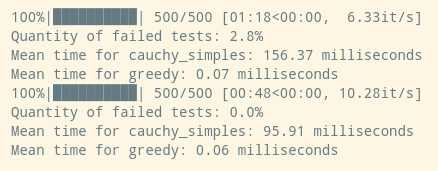
\includegraphics[width=4in]{theory_tester/theory_images/results_compare.png}
\caption{Результаты сравнения алгоритмов CauchySimplex и StandardGreedy}
\label{fig:comparison_standard_greedy_cauchy_simplex}
\end{figure}

\section{Параметры}

Набор используемых семейств распределений дан в таблице \ref{table:aversion_distribution_family}. Число $a$ для каждого рычага сэмплируется из $\mathcal{N}(1,1)$ (за исключением градиентных бандитов, чтобы продемонстрировать их невосприимичвость к изменению среднего). Параметр растяжения $\sigma$ для каждого рычага был взят из $\sigma \sim Exp(2)$. Таким образом, при $\nu > 2$ дисперсия каждого рычага равна $\sigma^2$. Чтобы включить среди рычагов ``безрисковые'' рычаги, после домножения на $\sigma$ каждое из распределений с вероятностью $\frac{1}{n}$ ($n=10$) домножалось на 0. Таким образом, с вероятностью примерно $1 - e^{-1} \approx 63\%$ среди рычагов есть хотя бы один с нулевой дисперсией. Хотя для $t_2$ цель максимизации $\sum_{i=1}^n p_i m_i - \lambda \sum_{i=1}^n p_i^2 \sigma_i^2$ некорректна, поскольку у $t_2$ нет дисперсии, можно вместо дисперсии $\sigma^2$ подставить параметр растяжения $\sigma_{\text{scale}}^2$, возведенный в квадрат, то есть пытаться найти $\sum_{i=1}^n p_i m_i - \lambda \sum_{i=1}^n p_i^2 \sigma_{i, \text{scale}}^2$. Естественно, вся разработанная до этого теория не работает для максимизации измененной величины.

Списки отдельных экспериментов с применяемыми в них стратегиями даны в таблицах \ref{table:aversion_greedy}, \ref{table:aversion_adaptive}, \ref{table:aversion_positive}, \ref{table:aversion_ucb}, \ref{table:aversion_gradient_bandits}. Кроме того, были протестированы $\epsilon$-greedy стратегии с $\epsilon=0.1$ и скорректированной дисперсией. Об этом подробнее в разделе~\ref{sec:correction_eps_greedy}. Список гиперпараметров дан в таблице \ref{table:classic_hyperparameters}.

В качестве метрик взяты:
\begin{enumerate}
    \item $\text{Regret} = \left( \sum_{i=1}^n p_i^* m_i - \lambda \sum_{i=1}^n (p_i^*)^2 \sigma_i^2 \right) - \left( \sum_{i=1}^n p_i Q_t(i) - \lambda \sum_{i=1}^n (p_i)^2 S_t^2(i) \right)$ -- среднее сожаление, где $\textbf{p}^*$ -- решение исходной задачи
    \item $\text{Regret}_{{\text{real}}} = \left( \sum_{i=1}^n p_i^* m_i - \lambda \sum_{i=1}^n (p_i^*)^2 \sigma_i^2 \right) - \left( \sum_{i=1}^n p_i m_i - \lambda \sum_{i=1}^n (p_i)^2 \sigma_i^2 \right)$ -- среднее реальное сожаление.
    \item Процент выбранных оптимальных действий на каждом шаге $Opt = 1 - 2 \sum_{i=1}^n |p_i - p_i^*|$. Заметим, что в обычной задаче о многоруких бандитах $P = (0, ..., 1, 0, ..., 0)$, и новая метрика равна 
    \[
    1 - \frac{1}{2}\left( (1 - b_k) + \sum_{i = 1, i \neq k}^n b_i \right) = 1 - (1 - b_k) = b_k
    \]
    то есть совпадает с процентом оптимальных действий, а это есть вторая метрика в обычной задаче о многоруких бандитах.
\end{enumerate}
В качестве вероятности $p$ в метрики будем подставлять ту вероятность, из которой в данный шаг происходит выбор рычага (то есть, например, для $\epsilon$-greedy, если выбор происходил случайно, то в метрику подставлялся вектор $\left( \frac{1}{n}, ..., \frac{1}{n} \right)$, хотя внутри себя стратегия хранит другое значение вероятностей). Выбор в пользу такого варианта был сделан, поскольку нам важно, на какие рычаги в реальности происходят нажатия, а не то, какая стратегия когда-то будет использоваться, то есть важна ``стоимость'' обучения. Для каждого распределения и каждой метрики результаты для одной группы стратегий визуализированы на графике. Кроме того, для каждой стратегии и для каждой метрики на одном графике были изображены результаты по всем распределениям.
 
Так как коэффициент отвращения к риску $\lambda$ также может влиять на эффективность алгоритмов, то будем дополнительно строить графики зависимости метрик от числа шагов для разных распределений и для одной фиксированной стратегии. Дополнительно построим график средних значений метрик на последних 5 шагах от $\lambda$ в зависимости от распределения, чтобы понять изменение конечного результата работы алгоритмов в зависимости от важности риска. Для оценки были взяты $\lambda \in [0.01, 0.05, 0.12, 0.3, 0.6, 1, 2, 4, 10]$.

\begin{table}
\centering
\renewcommand{\arraystretch}{1.5}
\begin{tabular}{ |m{4cm}||m{2.1cm}|m{6cm}|  }
 \hline
 \multicolumn{3}{|c|}{Список используемых распределений} \\
 \hline
 Распределение & Обозначение & Плотность $p(x)$ \\
 \hline
  Нормальное   &  $t_{\infty} $&  $\frac{1}{\sqrt{2\pi \sigma^2}}e^{\frac{(x-a)^2}{2\sigma^2}}$ \\
 \hline
 Стьюдента с $\nu=3$ нормированное & $t_{3}$ & $\frac{1}{\sqrt{3}} \cdot \frac{2}{\pi \sqrt{3\sigma^2} \left( 1 + \frac{(x-a)^2}{3\sigma^2} \right)^2}$ \\
 \hline
 Стьюдента с $\nu=2.1$ нормированное & $t_{2.1}$ & $\frac{1}{\sqrt{21}} \cdot \frac{\Gamma(1.55)}{\sqrt{2.1 \pi \sigma^2} \Gamma(1.05)} \left( 1 + \frac{(x-a)^2}{2.1 \sigma^2} \right)^{-1.55}$ \\
 \hline
 Стьюдента с $\nu=2$ & $t_2$ & $\frac{1}{2\sqrt{2\sigma^2} \left( 1 + \frac{(x-a)^2}{2\sigma^2} \right)^{3/2}}$ \\
 \hline
\end{tabular}
\caption{Список семейств распределений для проверки стратегий в измененной задаче о многоруких бандитах. Рычаги каждый раз берутся из одного семейства.}
\label{table:aversion_distribution_family}
\end{table}


\begin{table}
\centering
\renewcommand{\arraystretch}{1.3}
\begin{tabular}{ |m{3cm}|m{5cm}|  }
 \hline
 \multicolumn{2}{|c|}{Тест $\epsilon$-greedy ($\forall a \hook Q_1(a) = \overline{R_1^2(a)} = 0$)} \\
 \hline
 Стратегия & Параметры \\
 \hline
  Жадная   &  $\epsilon = 0$ \\
 \hline
 $\epsilon$-жадная & $\epsilon = 0.01$ \\
 \hline
 $\epsilon$-жадная & $\epsilon = 0.1$ \\
 \hline
\end{tabular}
\caption{Параметры для теста жадной и $\epsilon$-жадной стратегий в измененной задаче}
\label{table:aversion_greedy}
\end{table}

\begin{table}
\centering
\renewcommand{\arraystretch}{1.3}
\begin{tabular}{ |m{3cm}|m{5cm}|  }
 \hline
 \multicolumn{2}{|c|}{Тест стратегий с адаптивным $\epsilon$ ($\forall a \hook Q_1(a) = \overline{R_1^2(a)} = 0$)} \\
 \hline
 Стратегия & Параметры \\
 \hline
 $\epsilon$-жадная & $\epsilon = 0.1$ \\
 \hline
 Adaptive-$\epsilon$   &  $\epsilon_0 = 1$ \\
 \hline
 Adaptive-$\epsilon$ & $\epsilon_0 = 10$ \\
 \hline
 VDBE & $\epsilon_0 = 1, \, \delta = 0.1, \, \tau = 1$ \\
 \hline
 VDBE & $\epsilon_0 = 10, \, \delta = 0.1, \, \tau = 1$ \\
 \hline
\end{tabular}
\caption{Параметры для теста стратегий с адаптивным $\epsilon$ в измененной задаче}
\label{table:aversion_adaptive}
\end{table}

\begin{table}
\centering
\renewcommand{\arraystretch}{1.3}
\begin{tabular}{ |m{4cm}|m{5cm}|  }
 \hline
 \multicolumn{2}{|c|}{Тест позитивной инициализации} \\
 \hline
 Стратегия & Параметры \\
 \hline
 $\epsilon$-жадная & $\epsilon = 0.1, \: \forall a \hook Q_1(a) = \overline{R_1^2(a)} = 0$ \\
 \hline
 Жадная оптимистичная & $\epsilon = 0, \: \forall a \hook x_0(a) = 6$ \\
 \hline
 $\epsilon$-жадная оптимистичная & $\epsilon = 0.1, \: \forall a \hook x_o(a) = 6$ \\
 \hline
\end{tabular}
\caption{Параметры для теста стратегий с позитивной инициализацией в измененной задаче}
\label{table:aversion_positive}
\end{table}

\begin{table}
\centering
\renewcommand{\arraystretch}{1.3}
\begin{tabular}{ |m{3cm}|m{4cm}|  }
 \hline
 \multicolumn{2}{|c|}{Тест UCB ($\forall a \hook Q_1(a) = \overline{R_1^2(a)} = 0$)} \\
 \hline
 Стратегия & Параметры \\
 \hline
 $\epsilon$-жадная & $\epsilon = 0.1$ \\
 \hline
 UCB & $c=2, \, \epsilon=0.001$ \\
 \hline
\end{tabular}
\caption{Параметры для теста UCB в измененной задаче}
\label{table:aversion_ucb}
\end{table}


\begin{table}
\centering
\renewcommand{\arraystretch}{1.3}
\begin{tabular}{ |m{4cm}|m{6cm}|  }
 \hline
 \multicolumn{2}{|c|}{Тест градиентных бандитов ($\forall a \hook Q_1(a) = \overline{R_1^2(a)} = 0, \, H_1(a) = 0, \, m_a \sim \mathcal{N}(5,1)$)} \\
 \hline
 Стратегия & Параметры \\
 \hline
 Градиентные бандиты & $\alpha=0.1, \text{baseline} = \bar{w_t}$ \\
 \hline
 Градиентные бандиты & $\alpha=0.1, \text{baseline} = 0$ \\
 \hline
 Градиентные бандиты & $\alpha=0.4, \text{baseline} = \bar{w_t}$ \\
 \hline
 Градиентные бандиты & $\alpha=0.4, \text{baseline} = 0$ \\
 \hline
\end{tabular}
\caption{Параметры для теста градиентных бандитов в измененной задаче}
\label{table:aversion_gradient_bandits}
\end{table}

\section{Результаты}

На всех результатах графики реального сожаления и процента оптимальных действий для распределения $t_2$ не имеет смысла ввиду отсутствия у распределения дисперсии.

\subsection{$\epsilon$-greedy}

В этом подходе получились следующие графики:

\begin{figure}[ht!] %!t
\centering
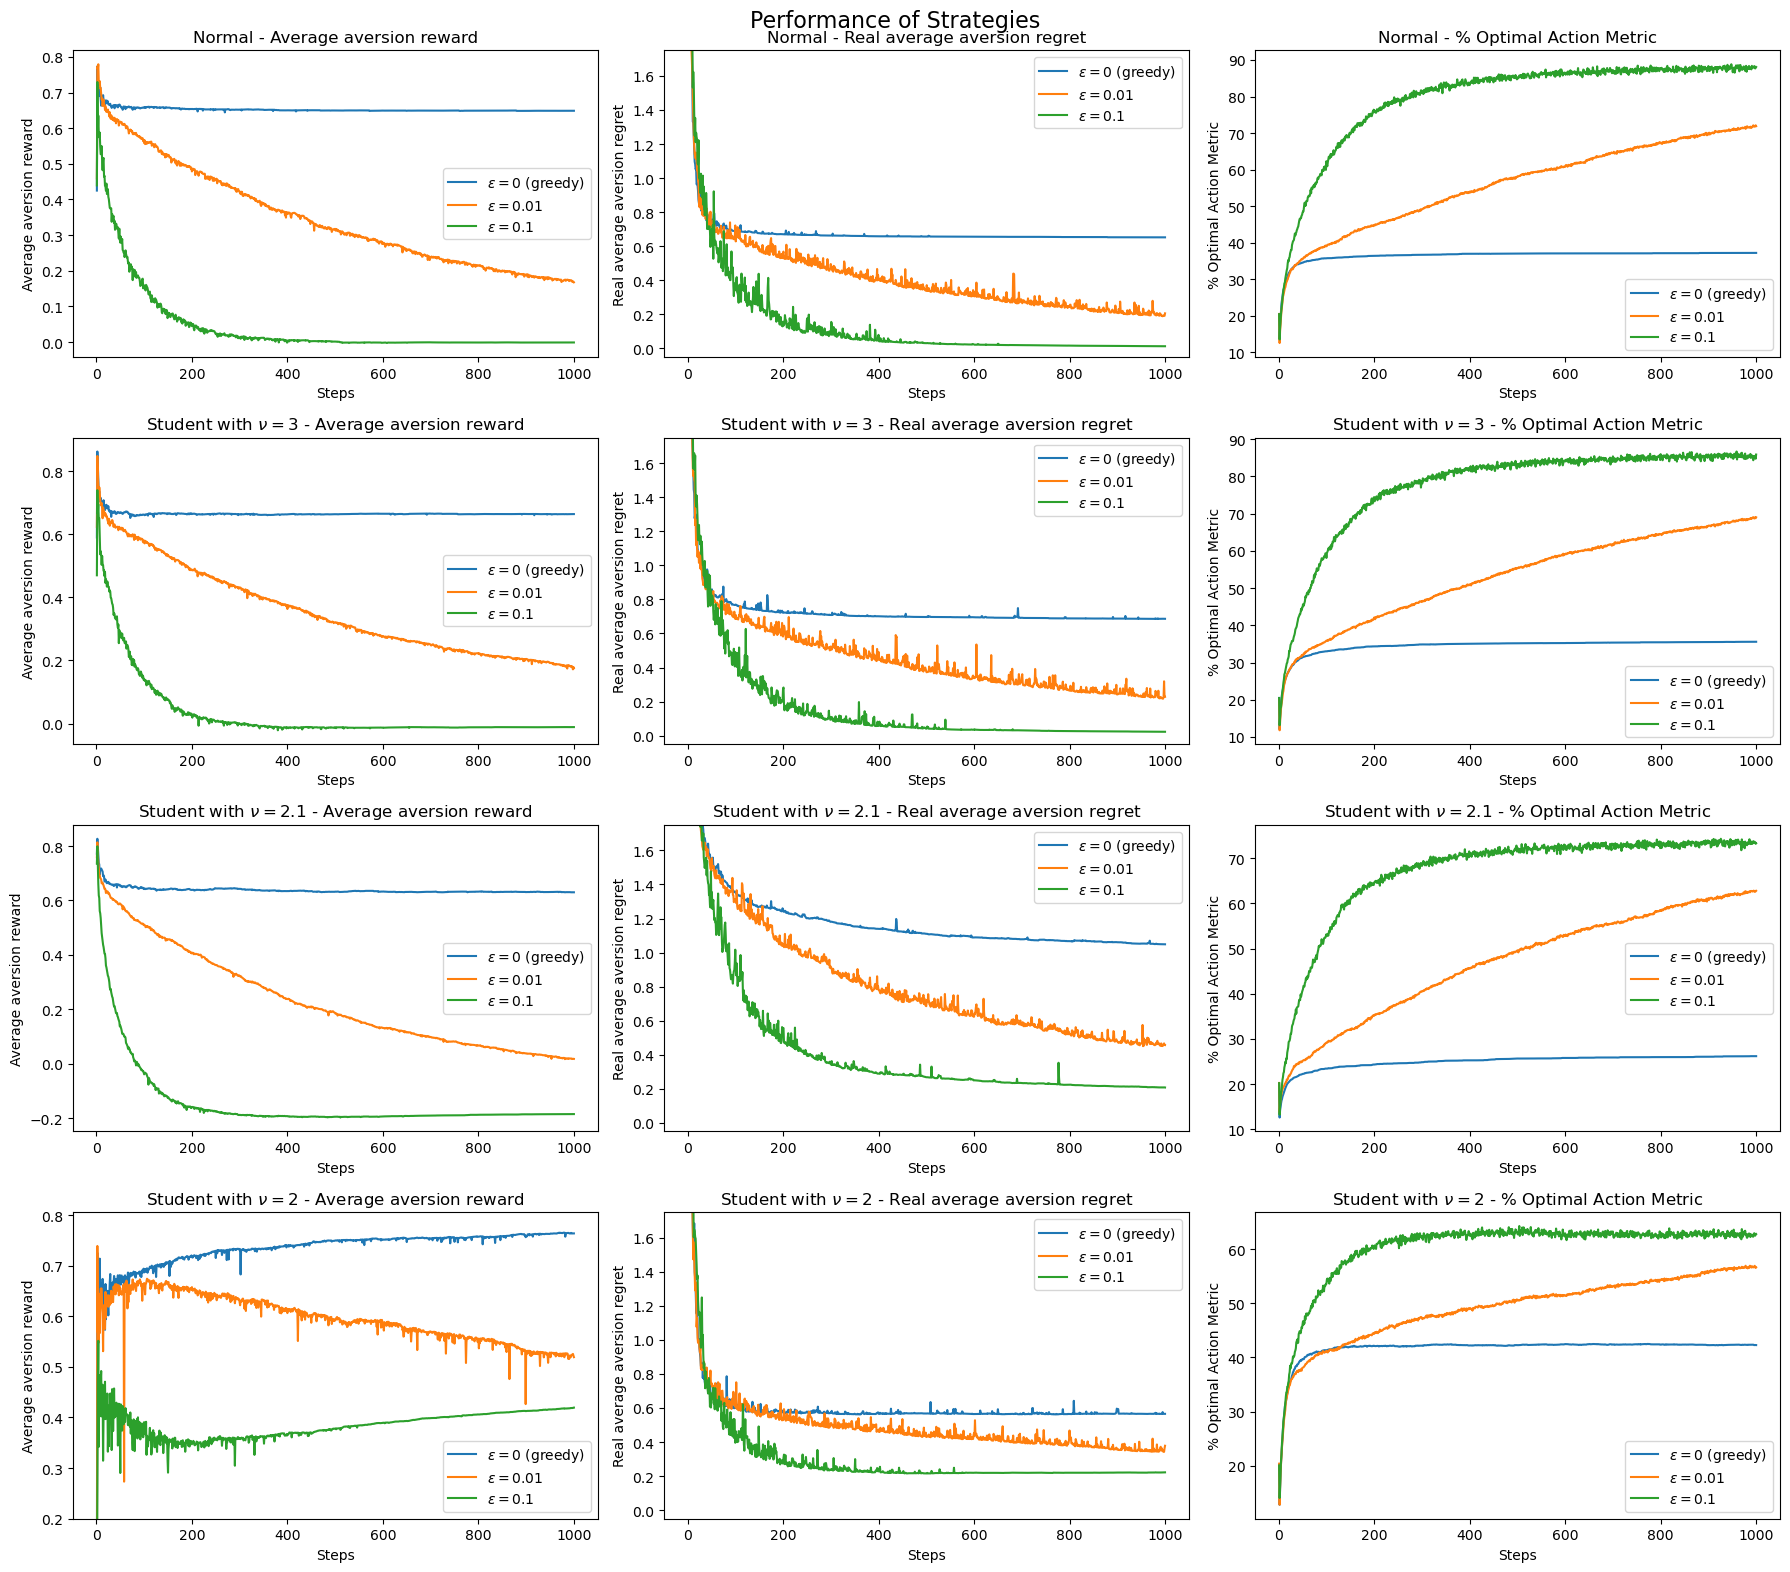
\includegraphics[width=6in]{theory_tester/theory_images/epsilon_greedy/strat_distr.png}
\caption{Зависимость метрик от количества шагов при greedy и $\epsilon$-greedy стратегиях для различных распределений}
\label{fig:epsilon_greedy_strat_distr}
\end{figure}

Хотя реальное сожаление не опускается ниже примерно $0.2$, алгоритм $\epsilon$-greedy выучивает с высокой точностью оптимальную стратегию, что можно видеть по следующему графику: 

Как можно видеть из \ref{fig:epsilon_greedy_strat_distr}, для любого распределения добавление случайного выбора улучшает exploration алгоритма, поэтому средние и дисперсии лучше приближаются, и ответ получается более близким к оптимальному. Например, для $t_{\infty}$ и $t_3$ и для $0.1$-greedy алгоритма процент оптимальных действий близок к $90\%$, почти достигая максимально возможного срднего значения в $91\%$. Также заметим, что для $t_{2.1}$ среднее значение сожаления Regret становится отрицательным, в то время как среднее реальное сожаление Regret$_{{\text{real}}}$ увеличилось на последних шагах до $0.4$ в отличие от $\approx 0.2$ для $t_3$. Это говорит о том, что алгоритм ``переоценивает'' себя, давая ``якобы'' лучше прибыль, чем оптимальное значения вероятности, из-за чего в реальности прибыль значительно ниже, чем для оптимальной вероятности.

Из-за чего это может происходить? Из-за недооценки значения дисперсии. Давайте смоделируем 10000 тестов, в каждом из них возьмем 1000 сэмплов из распределения Стьюдента с $t_{\nu}$ с дипсерсией 1, посчитаем выборочную дисперсию, а затем среди полученных 10000 выборочных дисперсий возьмем медиану. Эта медиана будет приближением медианы распределения выборочной дисперсии $s_{1000}^2$. Построим график зависимости этой медианы от числа степеней свободы при $\nu > 2$. Если бы мы считали выборочное матожидание вместо дисперсии, то ее медиана была бы постоянной и равнялась бы матожиданию $t_{\nu}$. В случае дисперсии все по-другому (см. \ref{fig:median_depend_on_df}):

\begin{figure}[ht!] %!t
\centering
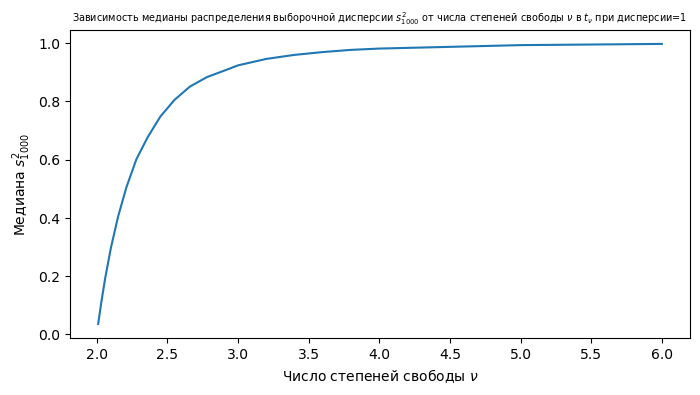
\includegraphics[width=5in]{theory_tester/theory_images/median_depend_on_df.png}
\caption{Зависимость медианы распределения выборочной дисперсии распределения Стьюдента $t_{\nu}$ относительно $\nu$}
\label{fig:median_depend_on_df}
\end{figure}

\begin{figure}[ht!] %!t
\centering
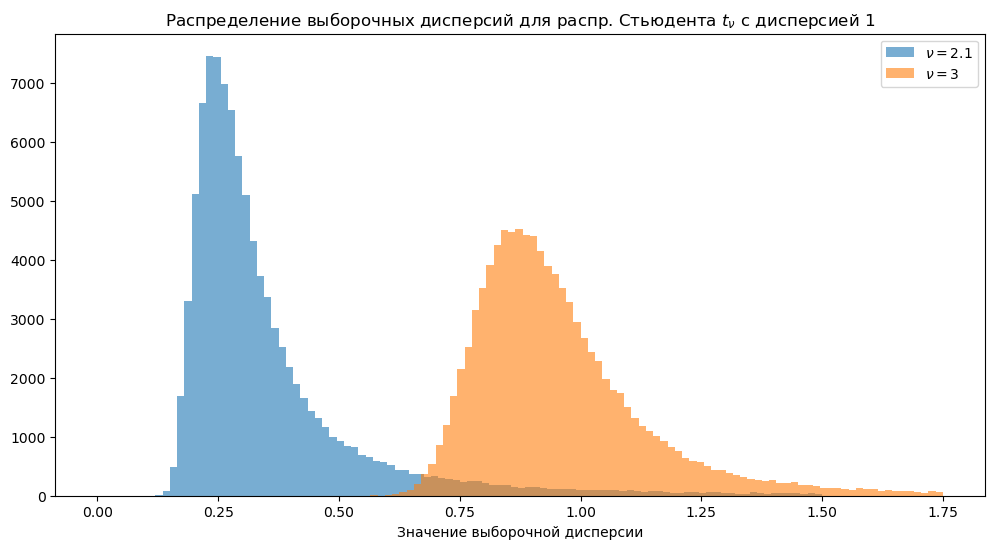
\includegraphics[width=5in]{theory_tester/theory_images/distributions_of_sample_variances.png}
\caption{Распределения выборочных дисперсий для распределений Стьюдента $\nu=2.1$ и $\nu=3$ с дисперсиями 1. Построено на 100000 значениях выборочной дисперсии $s_{1000}^2$}
\label{fig:distributions_of_sample_variances}
\end{figure}

Как можно видеть, медиана стремится к 0 при $\nu \to 2+$. При этом для любого $\nu$ медиана меньше среднего и медиана стремится к 1 при $\nu \to \infty$. В частности, при $\nu=2.1$ медиана примерно равна $0.3$, а при $\nu=3$ -- примерно равна $0.92$ (см. \ref{fig:distributions_of_sample_variances})

Это значит, что в большинстве случаев алгоритм недооценивает реальное значение дисперсии, из-за чего алгоритм склонен недооценивать риски и сосредотачивать деньги в активе с самой большой прибыльностью. А это, в свою очередь, снижает эффективность алгоритма. \label{negative_regret} Кроме того, поскольку дисперсии недооцениваются, то из прибыли вычитается меньшее значение, и потому алгоритм выдает большее значение прибыли, чем для оптимальной вероятности, что дает отрицательное среднее сожаление.

Что касается распределения Стьюдента $t_3$, то для него медианное значение дисперсии близко к реальному, поэтому эффект ``переоценки'' практически не проявляется.

Как мы выяснили, среди нарисованных на графике стратегий лучше всех работает $0.1$-greedy. Построим для нее график зависимости метрик от коэффциента отвращения для каждого распределения (\ref{fig:aversion_last_5_steps}):

\begin{figure}[ht!] %!t
\centering
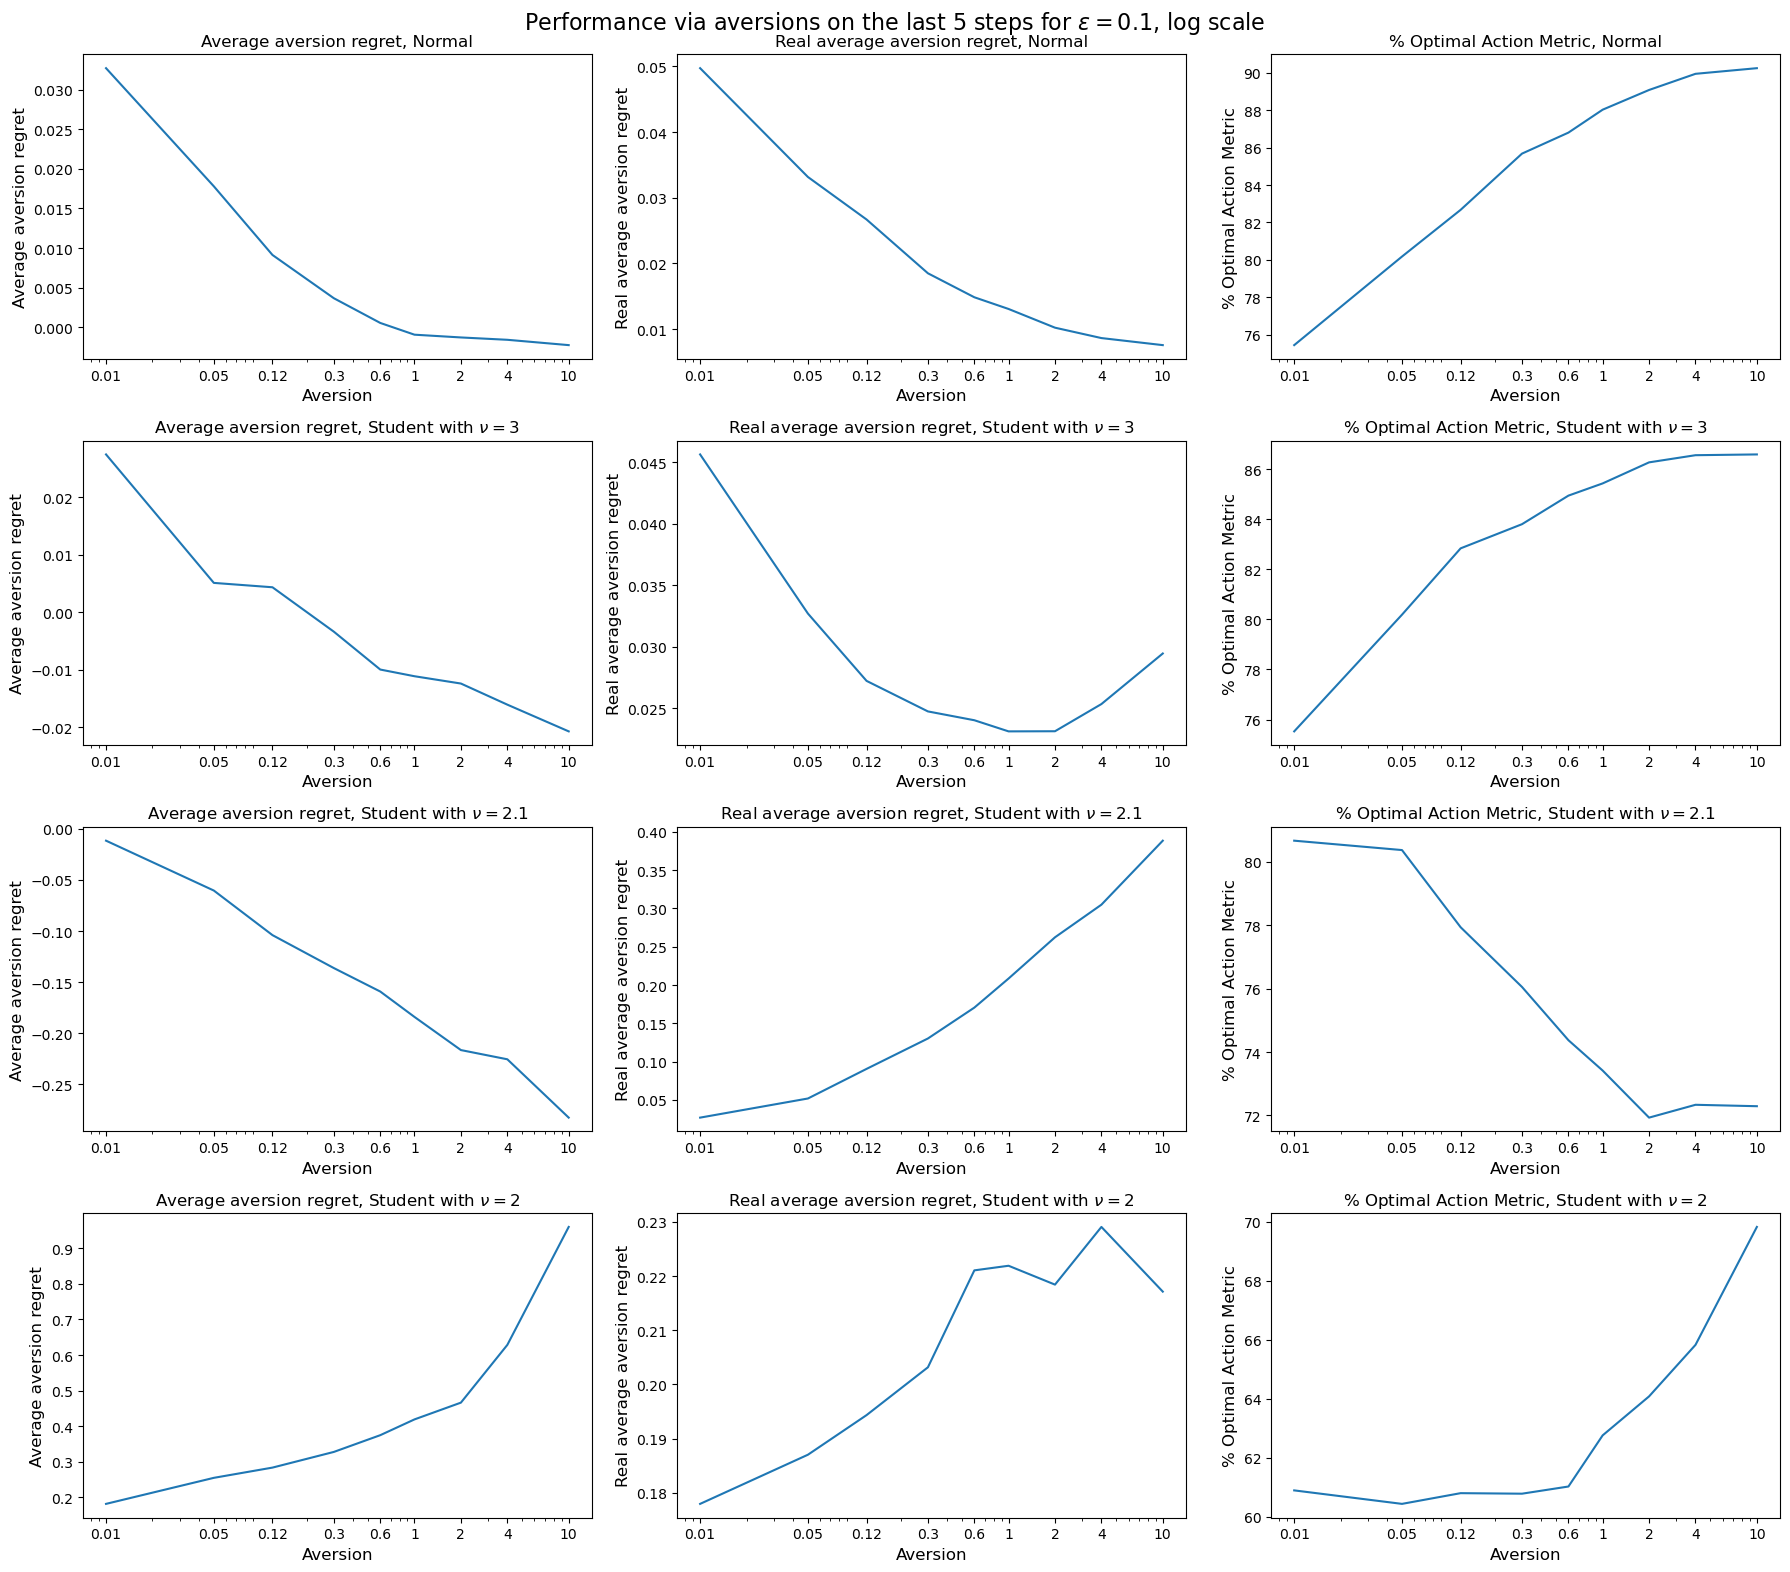
\includegraphics[width=6in]{theory_tester/theory_images/epsilon_greedy/aversion_last_5_steps.png}
\caption{График зависимости метрик от коэффциента отвращения для каждого распределения, усредненное по последним 5 шагам.}
\label{fig:aversion_last_5_steps}
\end{figure}

Как видно из графиков, для любого распределения с $\nu > 2$ при увеличении коэффициента отвращения к риску $\lambda$ метрика Regret уменьшается, и алгоритм переходит от своей недооценки к переоценке. Для $t_3$ и $t_{\infty}$ при увеличении $\lambda$ процент оптимальных действий увеличивается (хотя при $\nu = 3$ Regret$_{{\text{real}}}$ имеет минимум). В какой-то момент происходит переход, и для $t_{2.1}$ при уменьшении $\lambda$ точность увеличивается. Для $t_2$ при уменьшении $\lambda$ тоже наблюдается уменьшение Regret$_{{\text{real}}}$.

Почему при $\lambda \to 0+$ для больших степеней свободы эффективность алгоритма падает? При маленьких $\lambda$ дисперсия почти не учитывается при подсчете формулы, поэтому в оптимальном векторе вероятностей вся вероятность находится в рычаге с наибольшим матожиданием. Возьмем 2 рычага с наибольшим матожиданием $L_1$ и $L_2$ (у $L_1$ матожидание больше). Предположим, что у $L_1$ больше дисперсия, чем у $L_2$ (вероятность этого $\approx 0.5$). Тогда флуктуация получаемых наград у $L_2$ будет больше, чем у $L_1$, а это приводит к тому, что часто случается ситуация, при которой $Q_t(L_1) < Q_t(L_2)$. В таком случае в $91\%$ случаев $0.1$-greedy алгоритм будет выбирать $L_2$, что далеко от оптимального действия нажимать на рычаг $L_1$. При увеличении $\lambda$ этот недостаток нивелируется более равномерным распределением вероятностей по рычагам и потому более частым выбором $L_1$.

При $\nu$, близких к 2, описанный выше эффект начинает нивелировать эффект недооценки (преуменьшения) дисперсии: при больших $\lambda$ вероятности более равномерно распределяются по рычагам. Но алгоритм оценивает дисперсию каждого рычага значительно меньше, чем есть на самом деле, поэтому алгоритм старается сильнее концентрировать вероятности в одном рычаге, что дает отличие в векторах вероятностей и итоговое уменьшение эффективности. Далее мы на других графиках увидим, что такое поведение связано именно с преуменьшением дисперсии.

Уменьшение метрики Regret на графике для $t_{\infty}$ связано с уменьшением точности алгоритма при уменьшении $\lambda$, а для $t_{3}$ и $t_{2.1}$ это, опять-таки, происходит из-за преуменьшения дисперсии, как было уже сказано ранее \ref{negative_regret}.

\begin{figure}[ht!] %!t
\centering
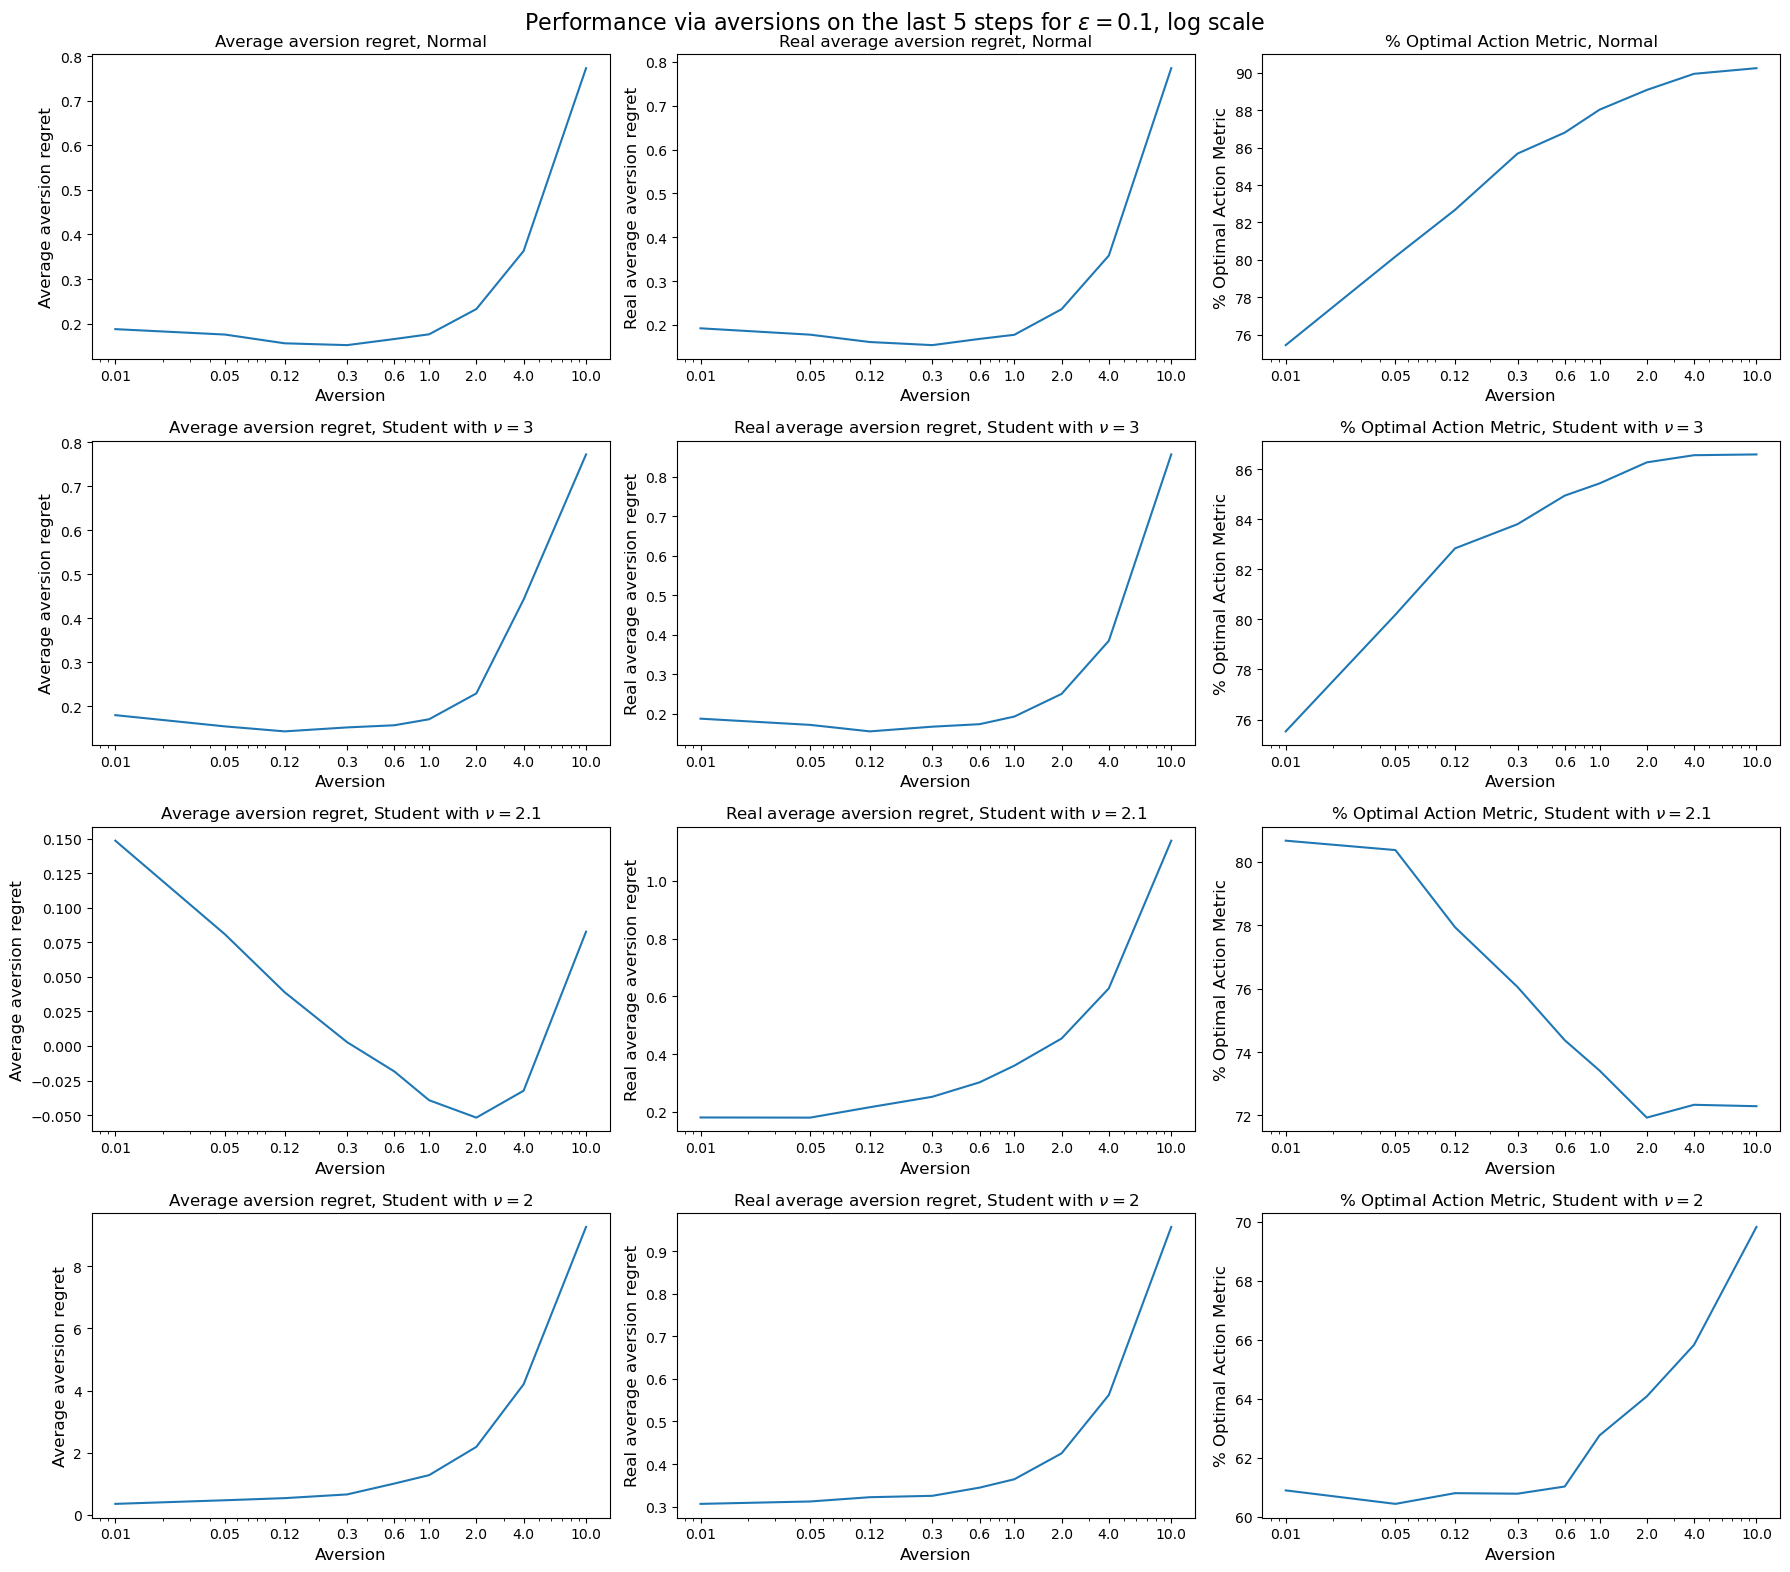
\includegraphics[width=6in]{experiments_aversion/eps_greedy/x_axis_aversion.png}
\caption{Графики зависимости метрик от количества шагов для каждого коэффициента отвращения.}
\label{fig:eps_greedy_aversion_selected_aversions}
\end{figure}

Что еще интересно, так это то, что при маленьком $\lambda$ эффективность для $t_{2.1}$ выше, чем для $t_3$ и $t_{\infty}$, но при увеличении коэффициента отвращения ситуация меняется, и  для $t_{2.1}$ метрики становятся хуже, чем для $t_3$ и $t_{\infty}$ (см. \ref{fig:eps_greedy_aversion_selected_aversions}). При больших $\lambda$, как было замечено выше, это связано с недооценкой дисперсии. При маленьких $\lambda$ дисперсия уже не играет при нахождении вероятностей никакой роли. Так в чем же дело? Стоит предположить, что дело в более остром пике у $t_{2.1}$: при нажатии на рычаг у $t_{2.1}$ выборочное матожидание ближе к настоящему матожиданию, чем у $t_3$ и $t_{\infty}$, что приводит к большей точности. Сама возможность приближения гарантируется числом $\epsilon$. Похожие рассуждения были приведены в параграфе \ref{subsec:classic_epsilon_greedy} про $\epsilon$-greedy стратегии в классической задаче о многоруких бандитах.

\subsection{Коррекция выборочной дисперсии}\label{sec:correction_eps_greedy}

Итак, как мы выяснили, в связи со смещенной влево (относительно матожидания) медианой у выборочного среднего $s_n^2$ алгоритм в большинстве случаев недооценивает реальную дисперсию распределения. Предположим, что алгоритму откуда-то стало известно семейство распределений, откуда генерируются активы. Модифицируем алгоритм, чтобы исправить описанную проблему.

Пусть алгоритм будет домножать выборочную дисперсию каждого распределения на определенную константу. Мы хотим домножить на такое число, чтобы произведение с большой вероятностью было близко к реальной дисперсии. Понятно, что при увеличении дисперсии в $\alpha$ раз распределение выборочной дисперсии тоже ``растягивается'' в $\alpha$ раз. Рассмотрим единичную дисперсию. Возьмем такие 2 варианта константы:
\begin{enumerate}
    \item $c_m = \frac{1}{m}$, где $m$ -- медиана распределения выборочной дисперсии $s_{1000}^2$ распределения с дисперсией $\sigma^2=1$ -- median correction.
    \item $c_{\mu} = \frac{1}{\mu}$, где $\mu$ -- мода распределения выборочной дисперсии $s_{1000}^2$ распределения с дисперсией $\sigma^2=1$ -- mode correction.
\end{enumerate}
Обе константы можно посчитать, сгенерировав $k$ выборок из $1000$ наград, где $k$ достаточно большое, посчитав в каждой выборке выборочную дисперсию, а затем среди полученных $k$ значений либо взять медиану, либо, взяв дискретизацию значений, посчитать среди них наиболее часто встречающееся. Взяв $k=5\cdot 10^{5}$ и дискретизацию по трем знакам после запятой, для $t_{2.1}$ были получены следующие значения: $c_m = 3.37269, \: c_{\mu} = 4.03226$. Подставим эти значения в алгоритм $\epsilon$-greedy с $\epsilon = 0.1$ и распределением $t_{2.1}$. При подсчете сожаления будем подставлять исправленную выборочную дисперсию. Сравним полученный результат с $0.1$-greedy алгоритмом без корректировки дисперсии.

\begin{figure}[ht!] %!t
\centering
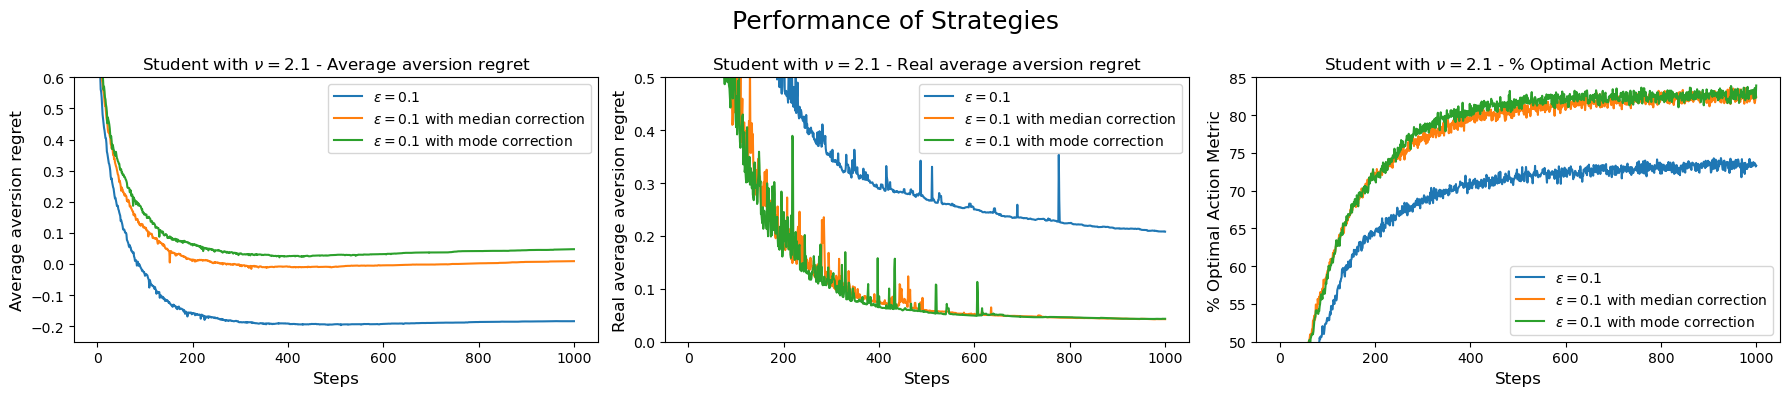
\includegraphics[width=6in]{theory_tester/theory_images/correction_variance/strat_distr.png}
\caption{Графики зависимости метрик от количества шагов для $t_{2.1}$ и стратегий с корректировкой выборочной дисперсии. Рассмотрена корректировка с помощью домножения на $c_m, \: c_{\mu}$ и без домножения (обычный $\epsilon$-greedy)}
\label{fig:aversion_correction_aversion_strat_distr}
\end{figure}

\begin{figure}[ht!] %!t
\centering
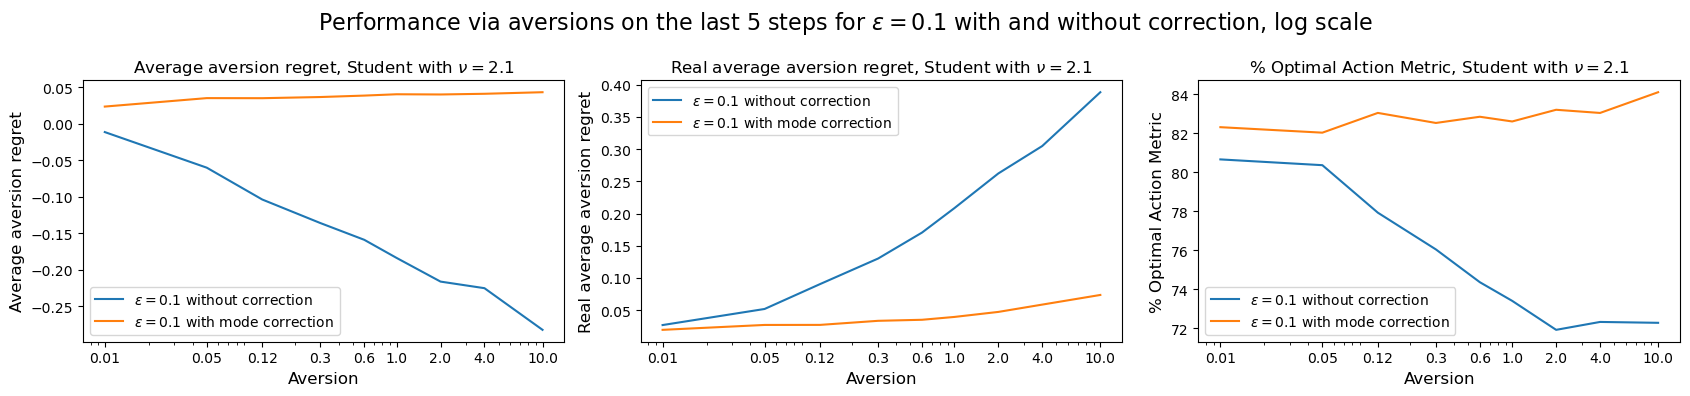
\includegraphics[width=6in]{theory_tester/theory_images/correction_variance/aversions_last_5_steps.png}
\caption{Графики зависимости метрик от коэффициента отвращения для $t_{2.1}$ и стратегий с корректировкой выборочной дисперсии. Рассмотрена корректировка с помощью домножения на $c_{\mu}$ и без домножения (обычный $\epsilon$-greedy)}
\label{fig:aversion_correction_last_5_steps}
\end{figure}

Как можно видеть, коррекция дисперсии значительно улучшает значения метрик. В частности, метрика Regret для стратегий с увеличением дисперсий не опускается ниже 0. Но процент оптимальных действий достигает максимального значения в примерно $85\%$, что меньше $90\%$, то есть у этих стратегий, при всех их преимуществах, устранены не все недостатки. Хотя у коррекций с помощью медианы и моды примерно одинаковые результаты, последняя все-таки незначительно лучше.

Оценим изменение значения метрик при различных коэффициентах отвращения для обычной $0.1$-greedy стратегии и для $0.1$-greedy стратегии с коррекцией с помощью моды.

Увеличение выборочной дисперсии практически устраняет с увеличением $\lambda$ ухудшение метрик Regret и Regret$_{\text{real}}$ и полностью устраняет уменьшение процента оптимальных действий. При этом в случае с процентом оптимальных действий можно наблюдать некоторое уменьшение метрик при $\lambda \to 0$, то есть начинает проявляться эффект неточности для двух рычагов с наибольшим матожмданием. В случае же Regret полномтью пропала переоценка стратегией самой себя. В целом же значения метрик для коррекции с помощью $c_{\mu}$ лучше, чем без коррекции при всех $\lambda$.

Хотя домножение дисперсии значительно улучшает эффективность стратегии, в реальной жизни это малоприменимо -- зачастую нам неизвестно число степеней свободы у распределения прибыли актива. Угадать константу, на которую нужно домножить, тоже не представляется возможным, поскольку значение медианы при $\nu > 2$ меняется от 0 до 1, и поэтому $c_m$ (и $c_{\mu}$) меняются от 1 до $\infty$ (см. \ref{fig:median_depend_on_df}).

\subsection{Адаптивный $\epsilon$-greedy}

Вернемся к стратегиям без коррекции дисперсии. Для стратегий с адаптивным $\epsilon$ получились следующие результаты (см. \ref{fig:adaptive_eps_strat_distr}):

Для всех распределений наилучшие результаты показали стратегии с начальным $\epsilon=10$. Это объясняется тем, что на начальных шагах у этих стратегий происходит фаза exploration, во время которой вероятности нажатий на рычаги распределены почти равномерно. Из-за этого дисперсии и матожидания приближаются более точно. Для $t_3$ и $t_{\infty}$ наилучший результат показала адаптивная $\epsilon$-greedy стратегия с $\epsilon=10$. Чуть хуже результаты у VDBE с $\epsilon=10$. Для $t_{2.1}$ эти стратегии показали примерно одинаковый результат. В отличие от $\epsilon$-greedy, адаптивные стратегии склонны к сильной переоценке своих результатов на начальных шагах (в то время как $\epsilon$-greedy, наоборот, недооценивает себя).

\begin{figure}[ht!] %!t
\centering
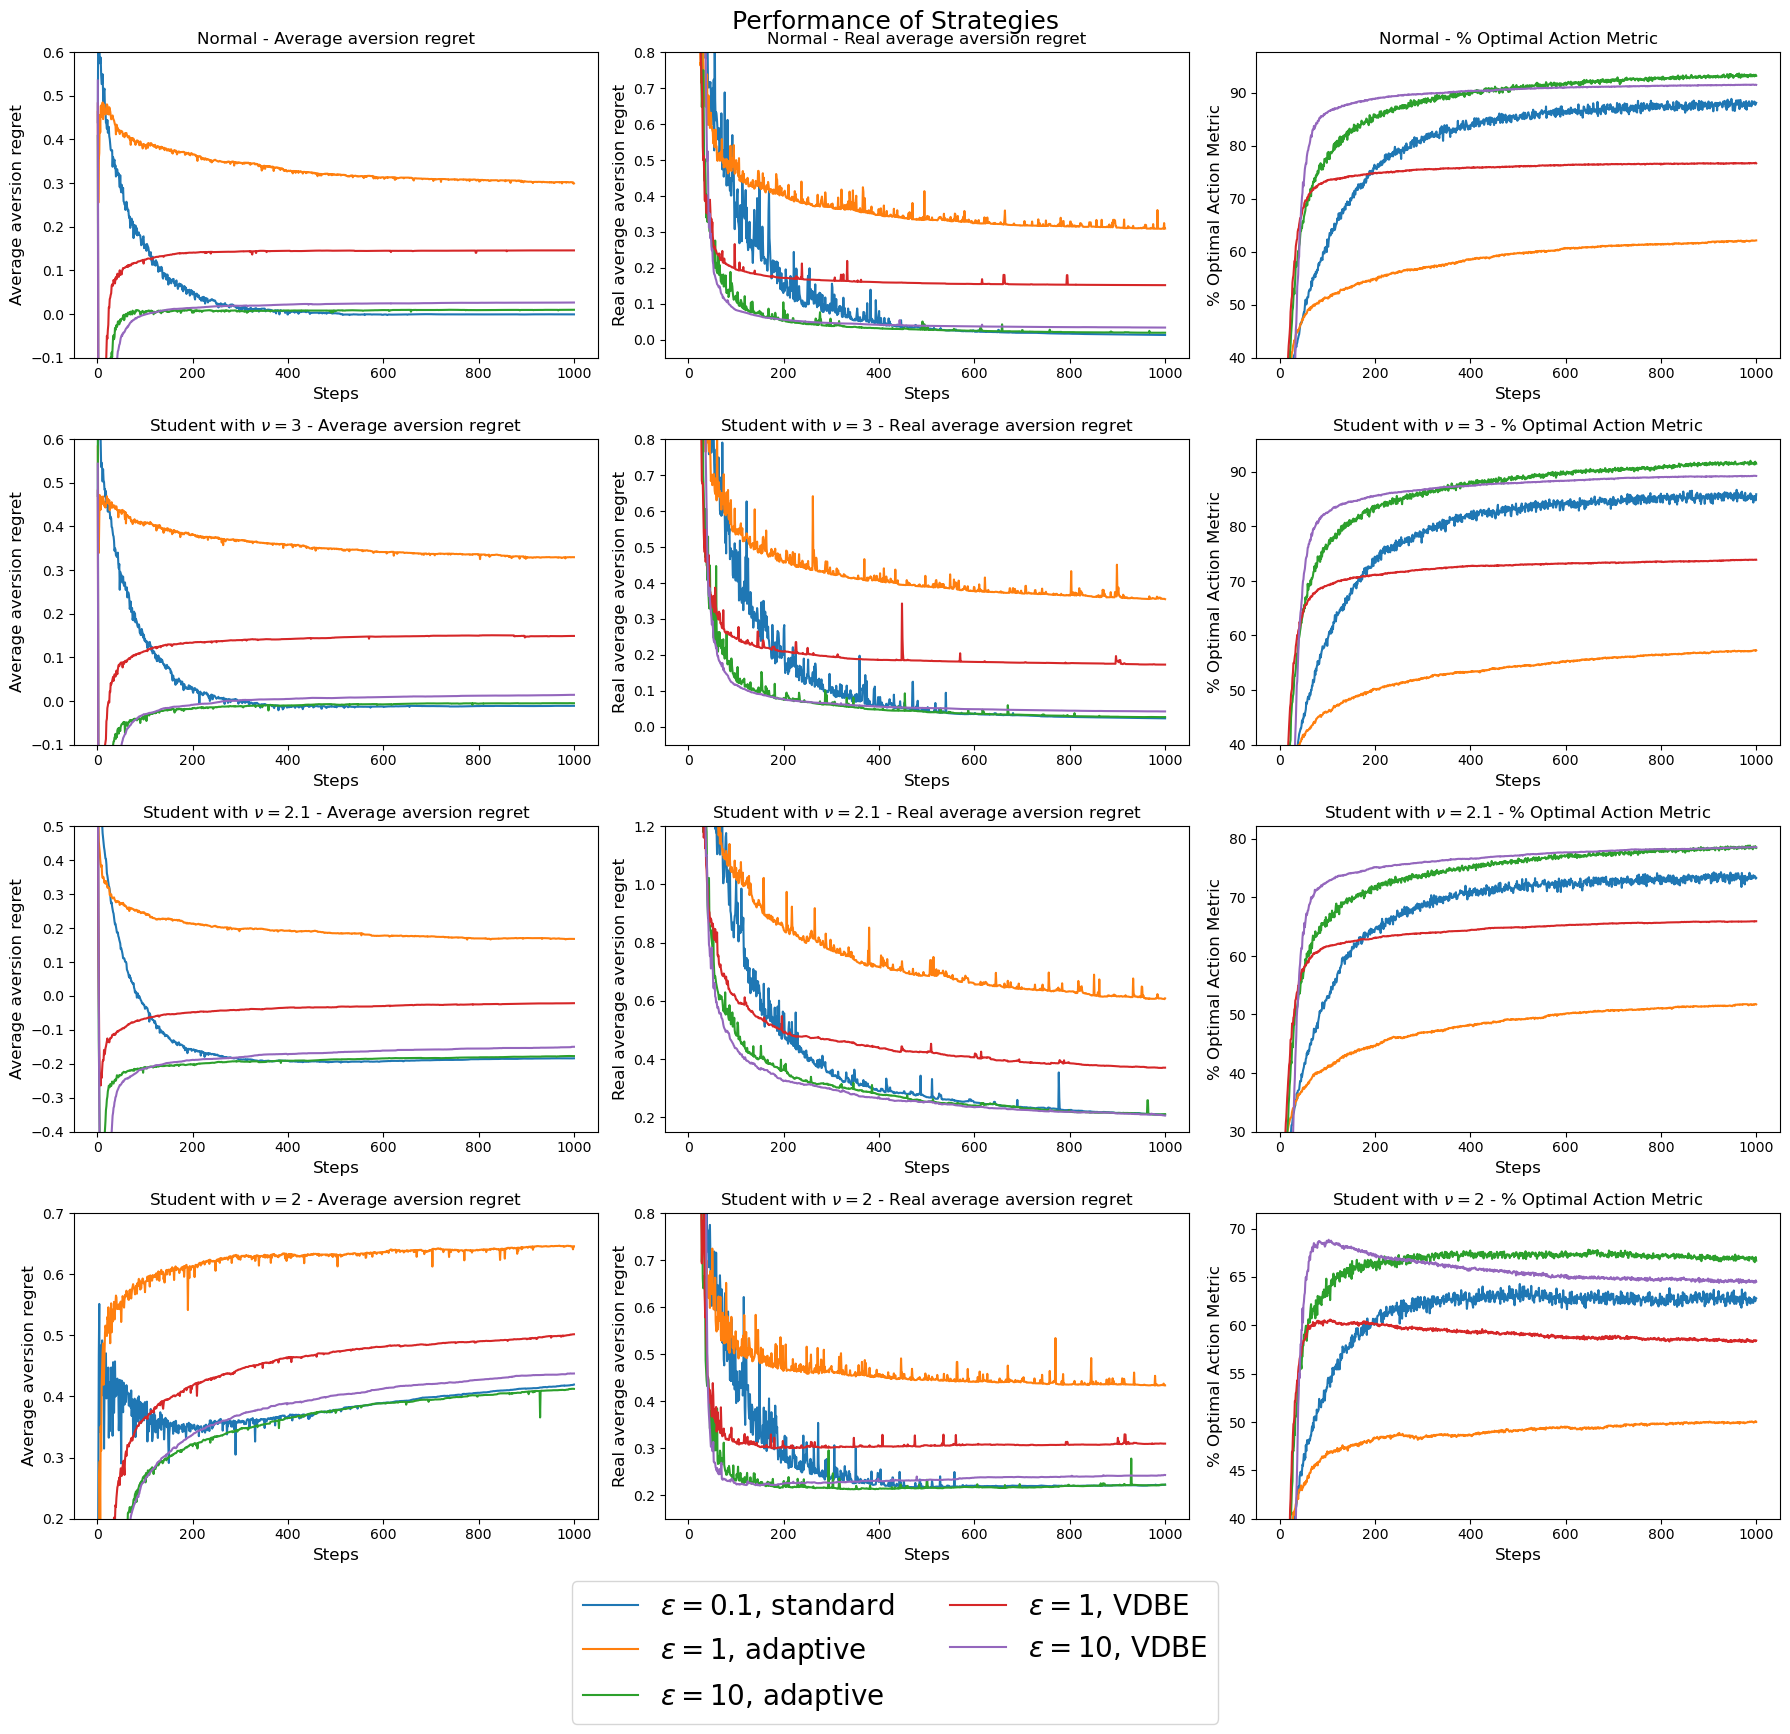
\includegraphics[width=6in]{theory_tester/theory_images/adaptive_epsilon/one_distr.png}
\caption{Зависимость метрик от количества шагов при $0.1$-greedy, adaptive-$\epsilon$ и VDBE стратегиях для различных распределений}
\label{fig:adaptive_eps_strat_distr}
\end{figure}

Поскольку стратегии с $\epsilon=10$ показали наилучший результат, посмотрим на изменение метрик для этих стратегий при различных коэффициентах отвращения:

\begin{figure}[ht!] %!t
\centering
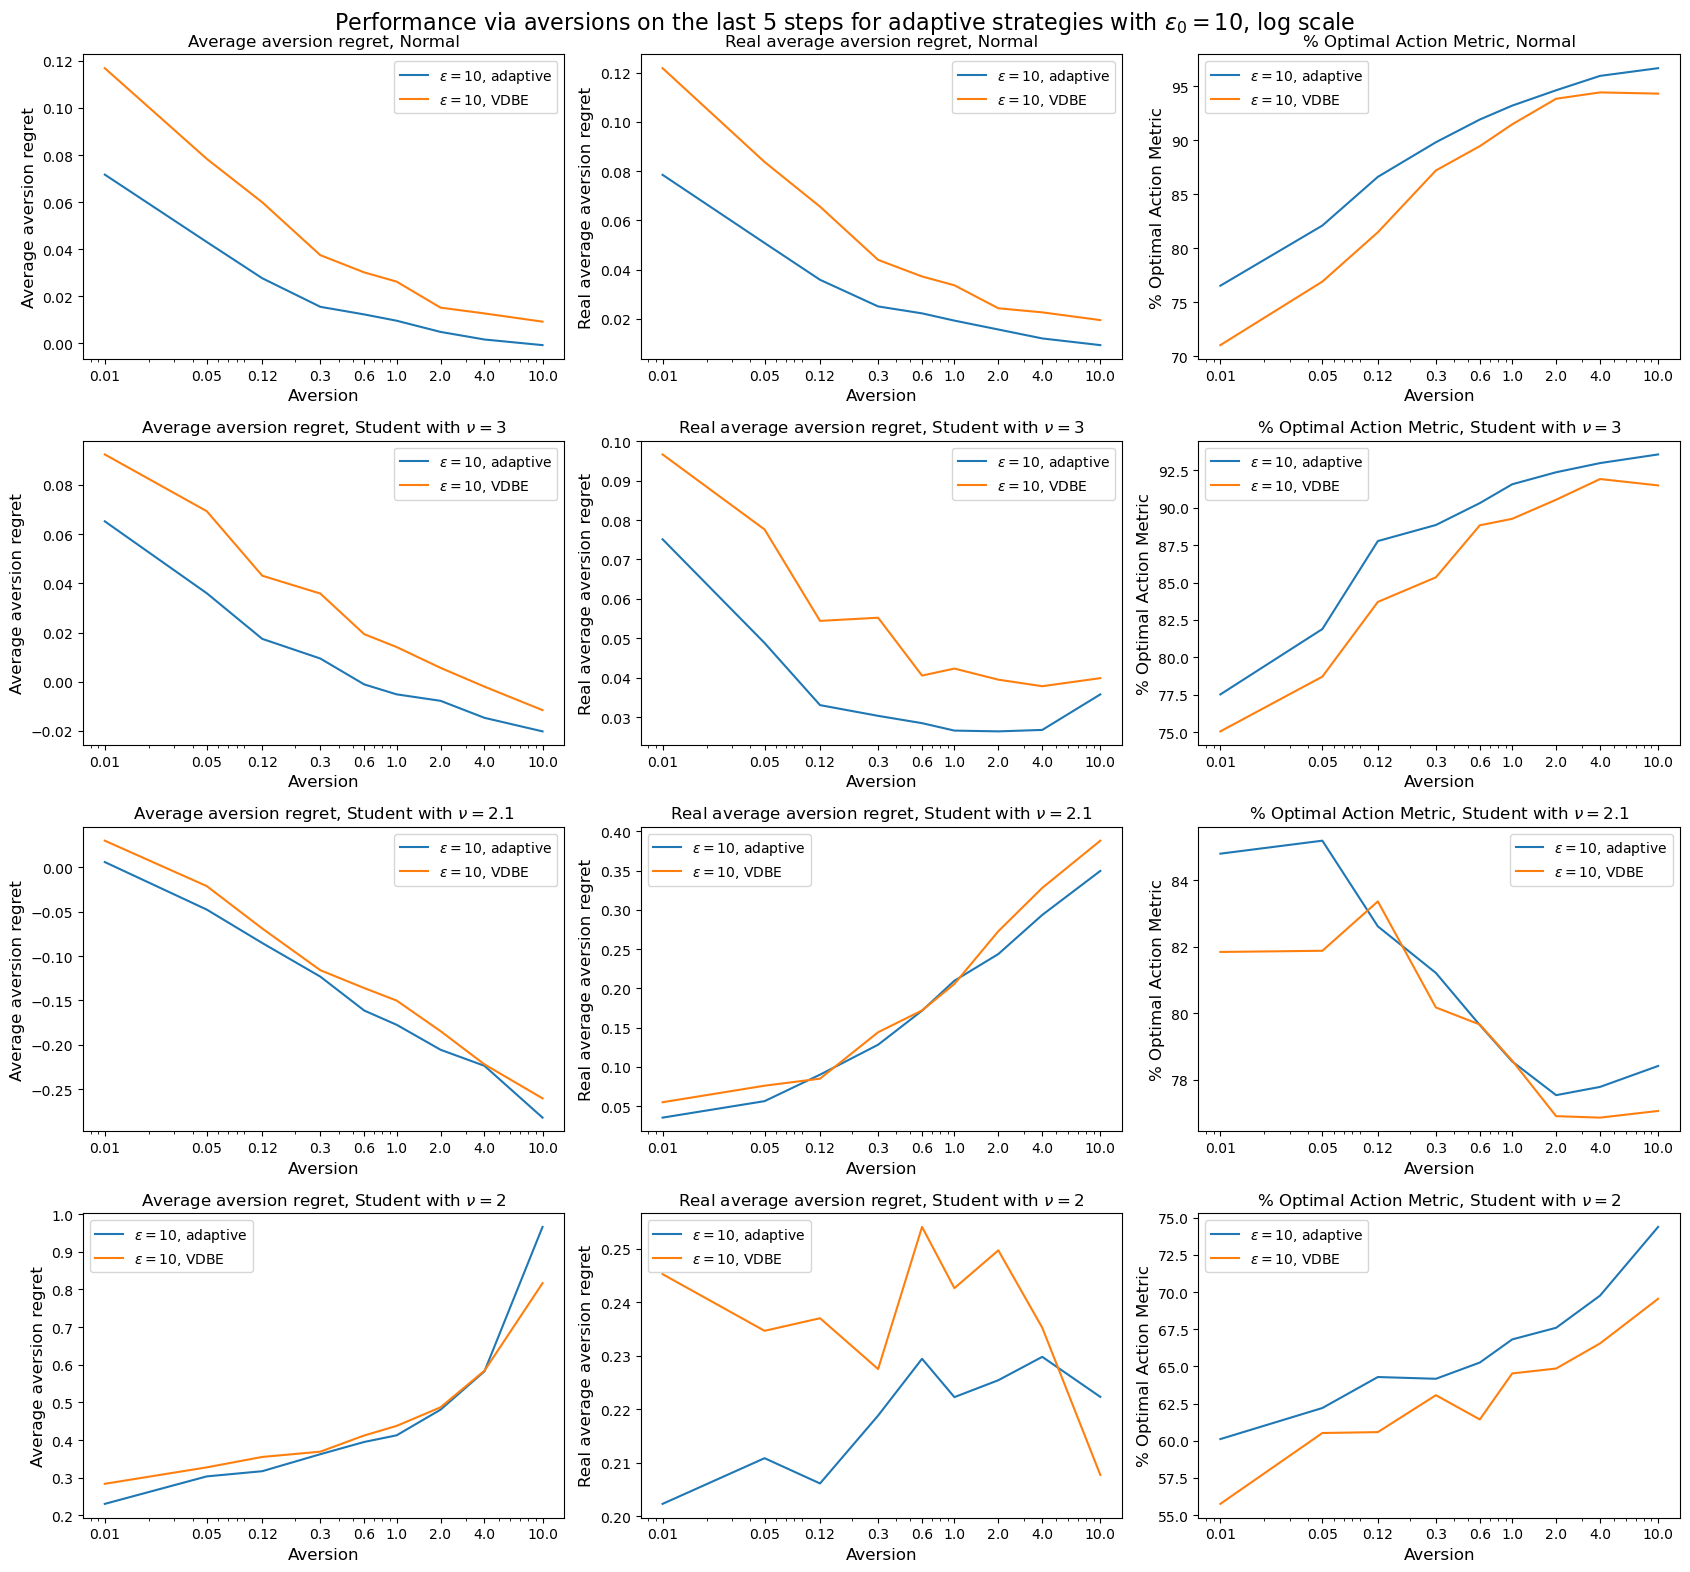
\includegraphics[width=6in]{theory_tester/theory_images/adaptive_epsilon/aversion_last_5_steps.png}
\caption{Графики зависимости метрик от коэффициента отвращения для $t_{2.1}$ и стратегий adaptive-$\epsilon$ и VDBE с $\epsilon=10$.}
\label{fig:adaptive_eps_last_5_steps}
\end{figure}

Как видно из \ref{fig:adaptive_eps_last_5_steps}, тенденция изменения метрик с изменением $\lambda$ схожа с таковой у $\epsilon$-greedy стратегии. Также стратегия adaptive-$\epsilon$ показывает себя лучше, чем VDBE. Однако VDBE обладает бОльшим потенциалом, поскольку позволяет настраивать дополнительные параметры -- температуру $\tau$ и шаг обновления $\delta$. Изучение поведения VDBE при различных параметрах $\epsilon$, $\tau$ и $\delta$ может быть интересной темой для дальнейших исследований.

\subsection{Позитивная инициализация}

Как было замечено ранее, для $t_{\nu}$ с $\nu > 2$ в обычной задаче о многоруких бандитах позитивная инициализация с постоянным step-size показывает результат лучше, чем $\epsilon$-greedy, при этом обучаясь до наибольших значений своих метрик за горяздо меньшее время. При этом у позитивной инициализации наблюдался эффект переобучения. Попробуем посмотреть на результаты этой стратегии в задаче с присутствием неприятия к риску.

\begin{figure}[ht!] %!t
\centering
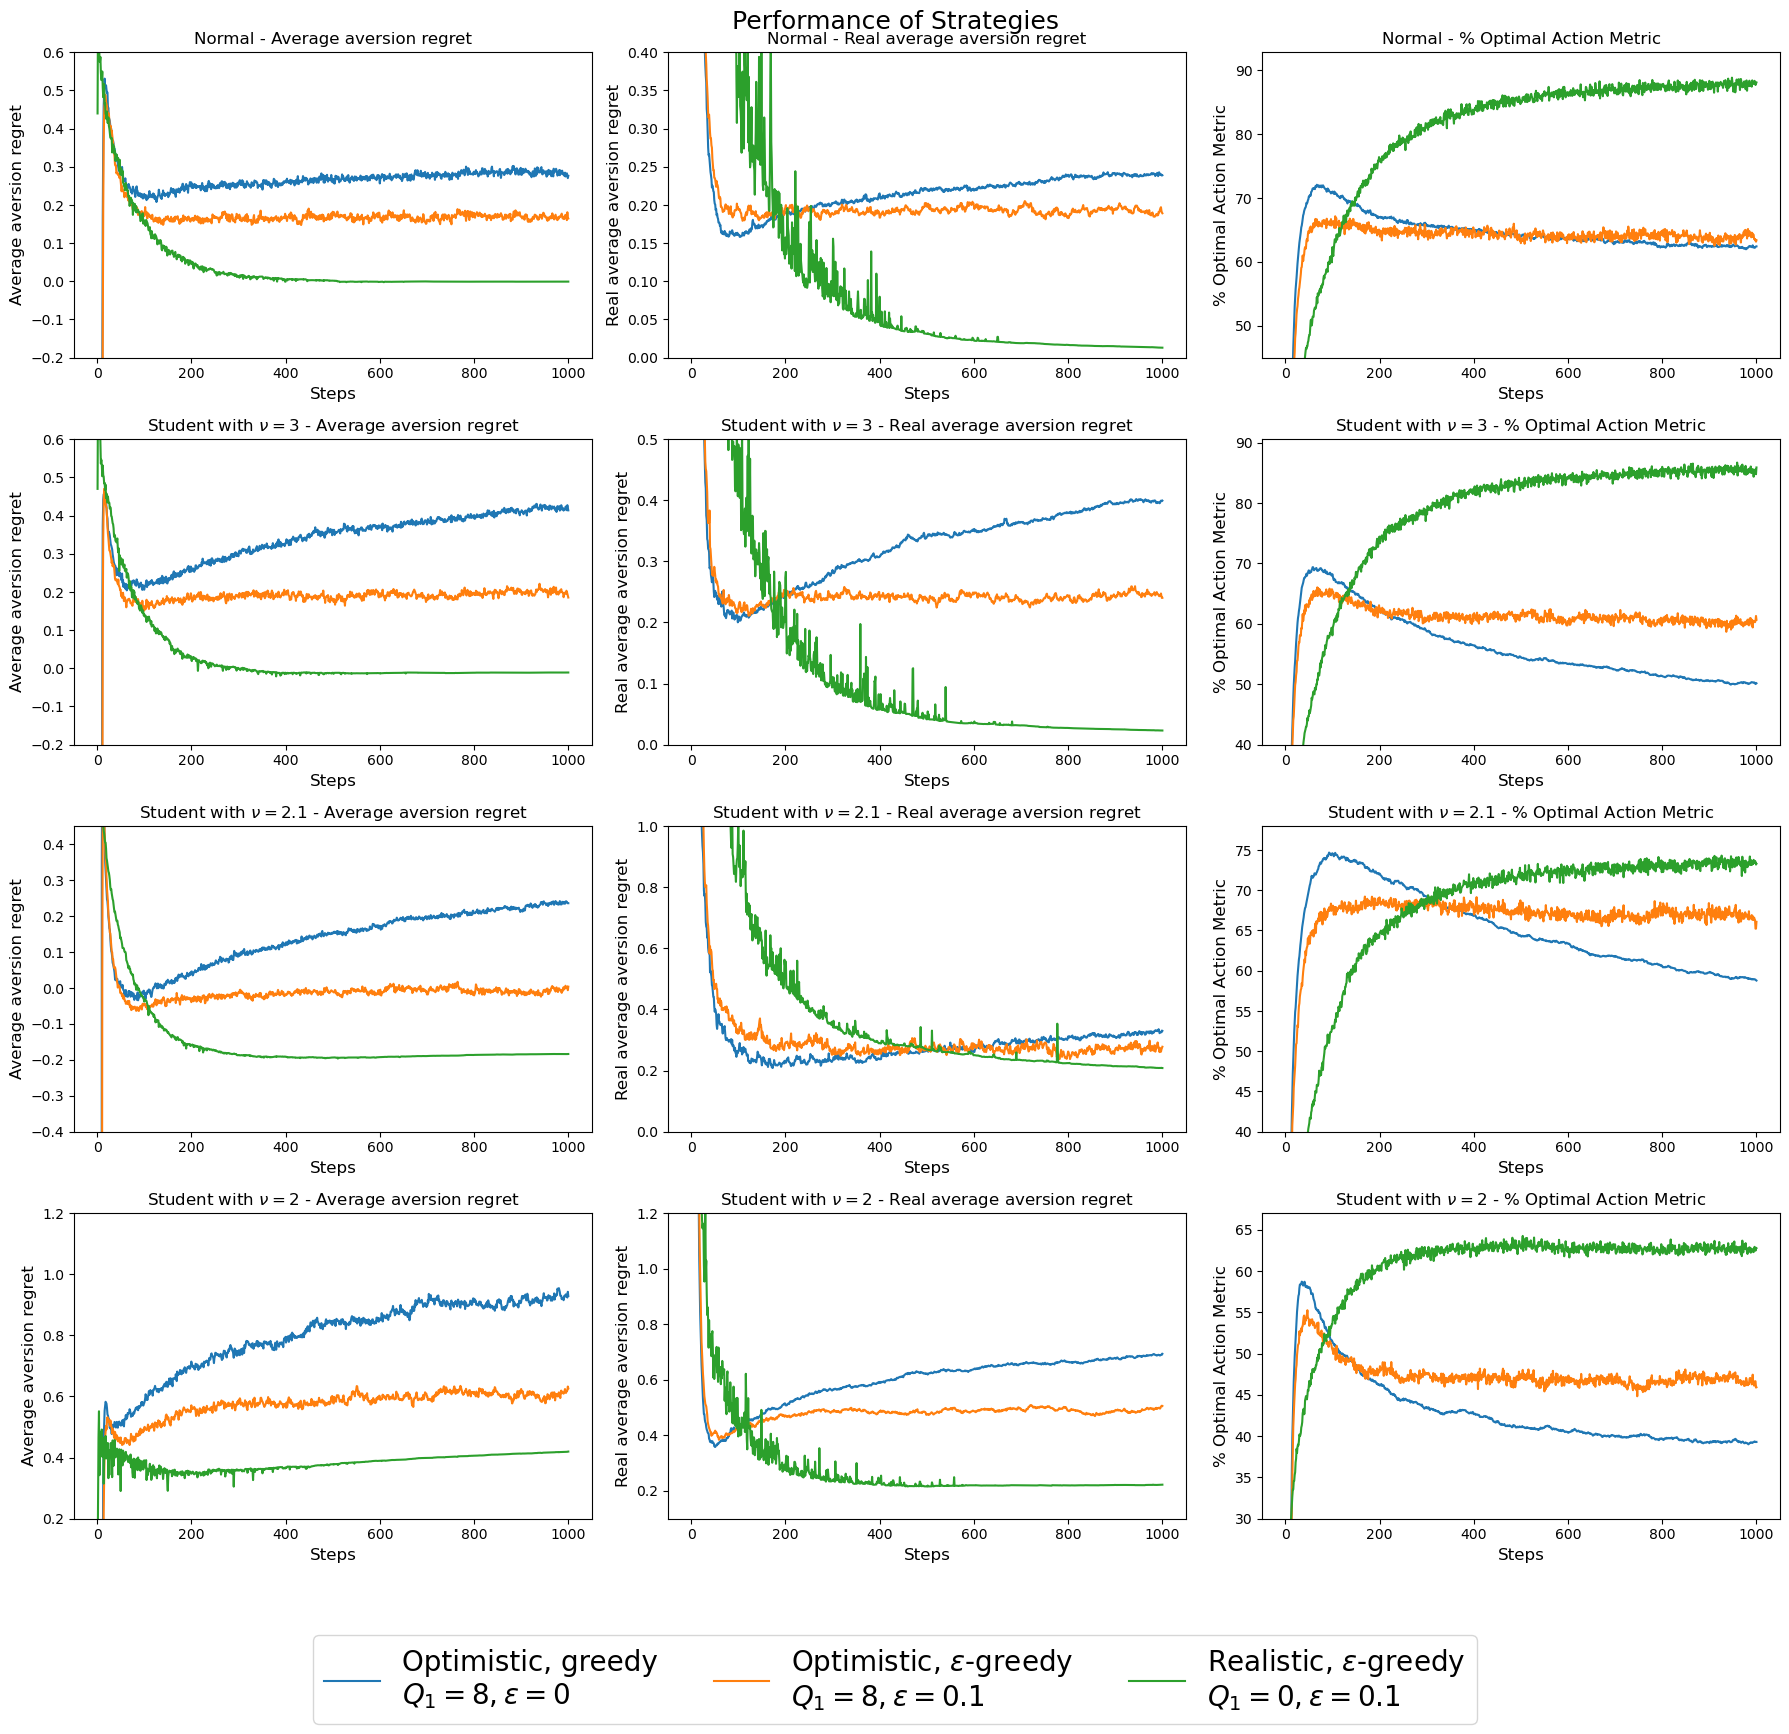
\includegraphics[width=6in]{theory_tester/theory_images/positive_init/one_distr.png}
\caption{Зависимость метрик для различных распределений от количества шагов при стратегиях с позитивной инициализацией, постоянным step-size и $\epsilon=0$ или $\epsilon=0.1$, а также при $0.1$-greedy стратегии}
\label{fig:positive_init_one_distr}
\end{figure}

Так же, как и в обычной задаче о многоруких бандитах, при позитивной инициализации наблюдается эффект переобучения. Однако в задаче о многоруких бандитах с учетом неприятия к риску эта стратегия превосходит $\epsilon$-greedy только для $t_{2.1}$. Несомненныи плюсом является то, что для достижения наилучших значений метрик позитивной инициализации понадобилось намного меньше шагов, чем $\epsilon$-greedy -- около 100 против 1000. Что еще интересно, так это то, что при $\lambda \to 2+$ наилучший процент оптимальных действий для жадной стратегии с позитивной инициализацией увеличивается (см. \ref{fig:positive_init_one_strat_positive_greedy}).

\begin{figure}[ht!] %!t
\centering
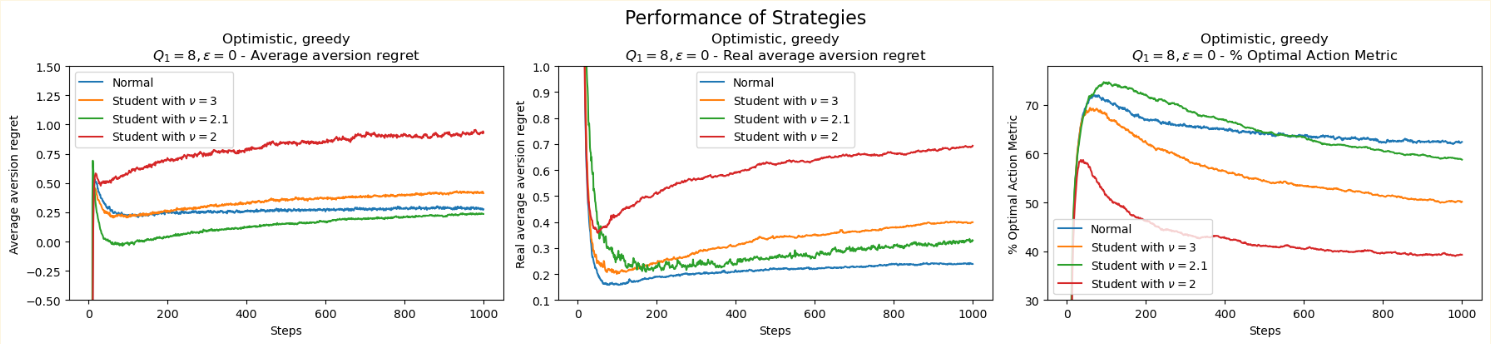
\includegraphics[width=6in]{theory_tester/theory_images/positive_init/one_strat_positive_greedy.png}
\caption{Зависимость метрик для различных распределений от количества шагов для жадной стратегии с позитивной инициализацией и постоянным step-size}
\label{fig:positive_init_one_strat_positive_greedy}
\end{figure}

\subsection{UCB}

В UCB изменению подверглось только выборочное матожидание, выборочную дисперсию изменения не тронули. Неудивительно, что UCB лишь незначительно улучшил результат для $t_{2.1}$, в остальных случаях показав ухудшение относително $0.1$-greedy (см. \ref{fig:ucb_compare_ucb_and_eps_greedy}).

\begin{figure}[ht!] %!t
\centering
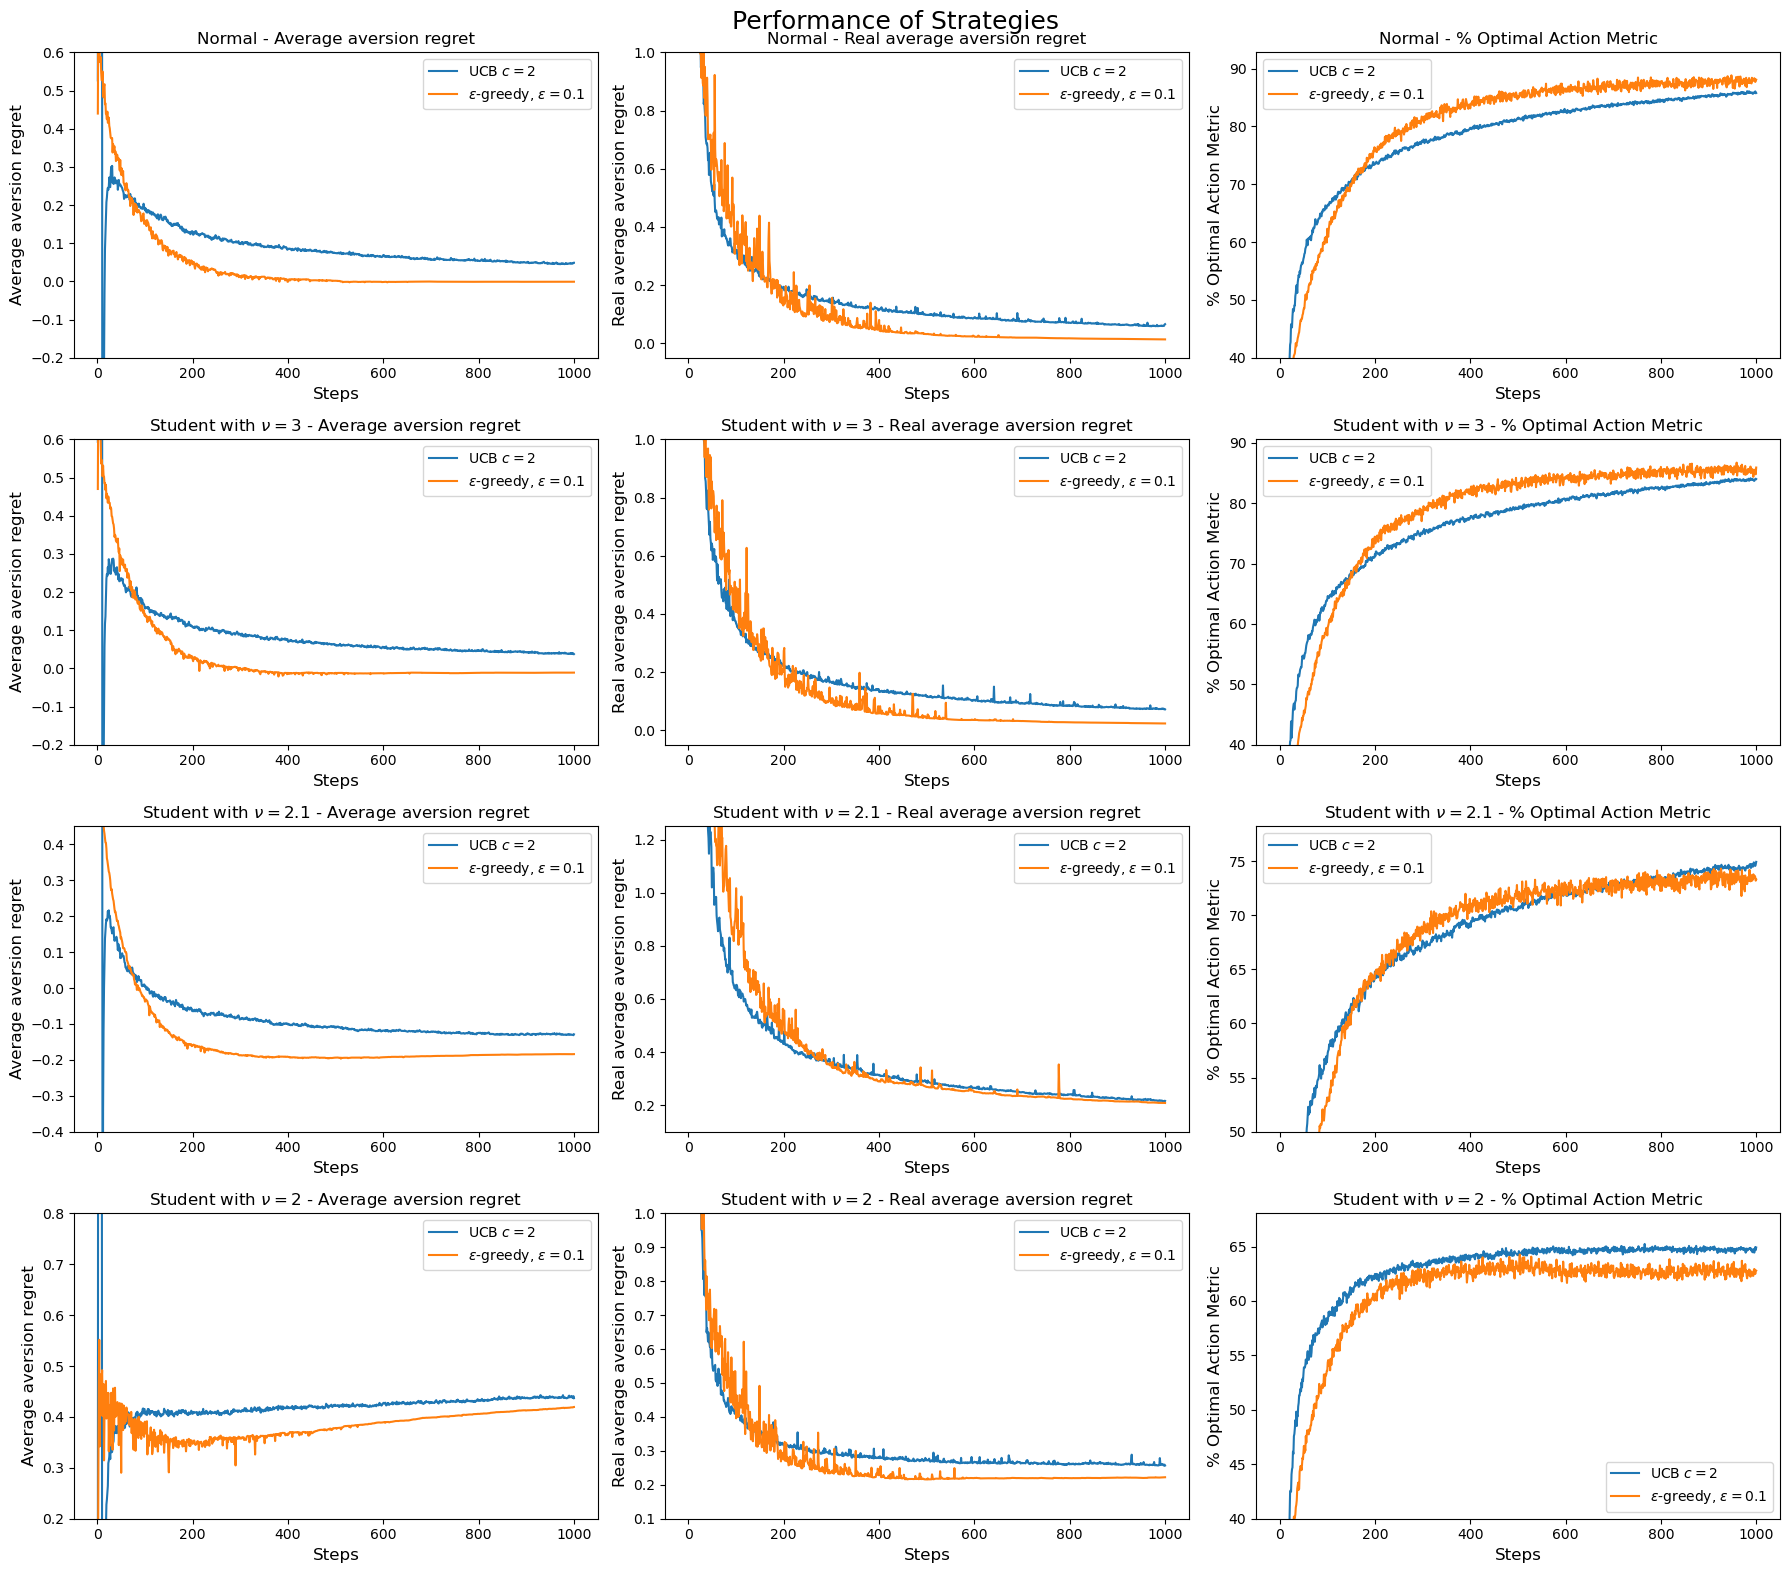
\includegraphics[width=6in]{theory_tester/theory_images/UCB/compare_ucb_and_eps_greedy.png}
\caption{Зависимость метрик для различных распределений от количества шагов для UCB с $c=2$ и $0.1$-greedy}
\label{fig:ucb_compare_ucb_and_eps_greedy}
\end{figure}

\begin{figure}[ht!] %!t
\centering
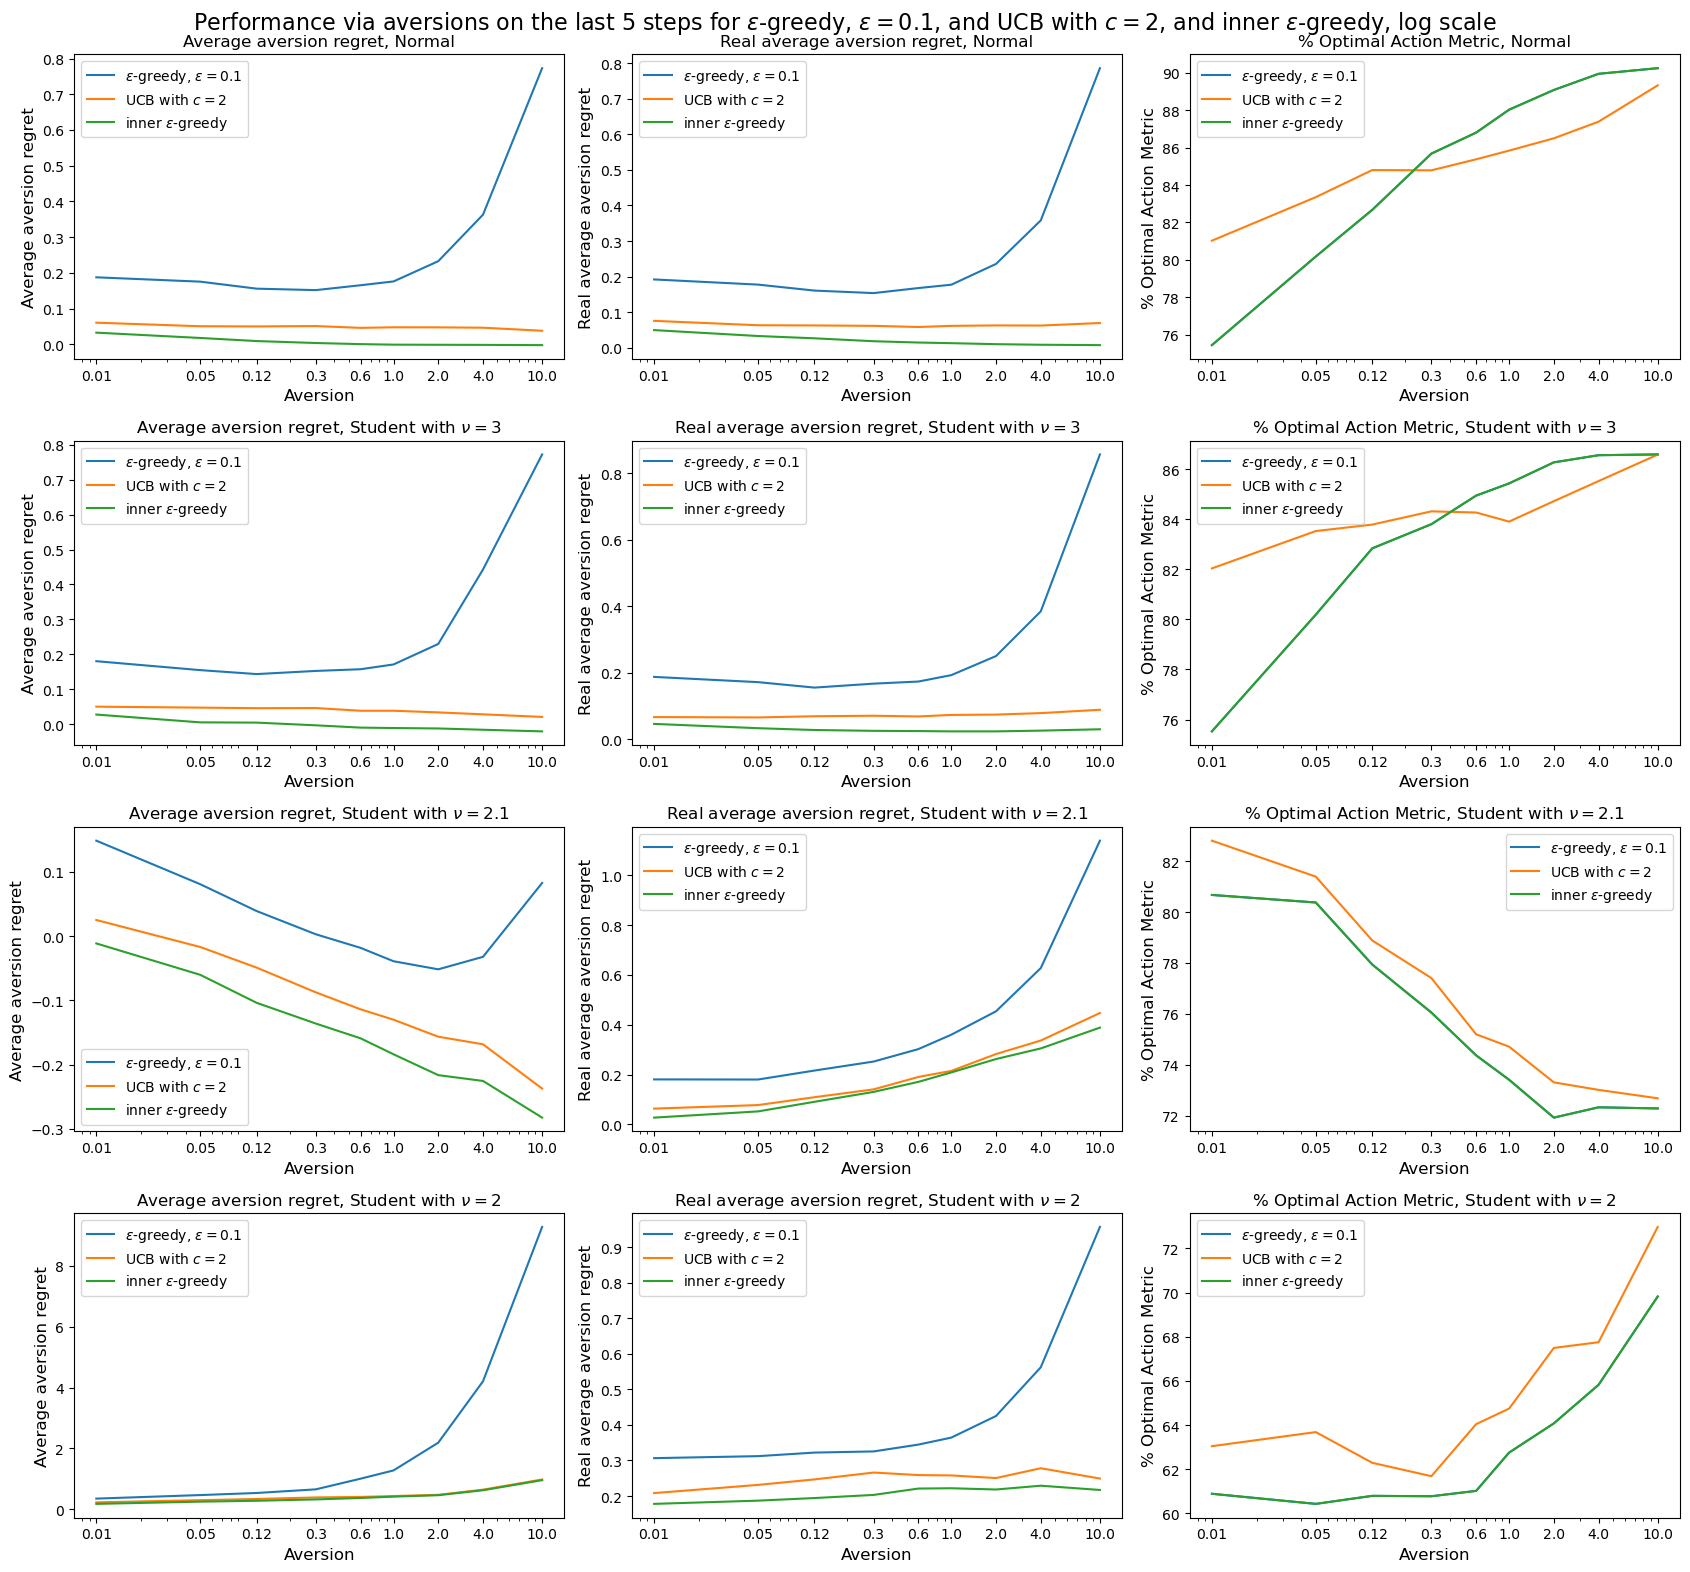
\includegraphics[width=6in]{Figures/experiments_aversion/ucb/last_5_steps.png}
\caption{Графики зависимости метрик от коэффициента отвращения для различных распределений и стратегий UCB с $c=2$, $\epsilon$-greedy и $\epsilon$-greedy с внутренней вероятностью}
\label{fig:ucb_compare_ucb_for_different_aversions}
\end{figure}

Однако, что интересно (\ref{fig:ucb_compare_ucb_for_different_aversions}), во-первых, для $t_{2.1}$ при любом $\lambda$ у UCB процент оптимальных действий выше, чем у $\epsilon$-greedy. Во-вторых, при маленьких $\lambda$ процент оптимальных действий у UCB выше, чем у $\epsilon$-greedy. Это объясняется тем, что прибавка вида $c\sqrt{\frac{\log t}{N_t(a)}}$ позволяет двум рычагам с наибольшими матожиданиями прожаться большее число раз, что дает лучшее приближение и, как следствие, лучший процент оптимальных действий. В-третьих, при всех $t_{\nu}$ и всех $\lambda$ значение метрики Regret$_{\text{real}}$ у UCB выше, чем у $\epsilon$-greedy (при том, что в некоторых случаях процент оптимальных действий лучше). После измерения дисперсий метрик оказалось, что дисперсии Regret$_{\text{real}}$ для UCB и $\epsilon$-greedy одинаковы. Такое странное поведение метрик можно объяснить большей рискованностью UCB: хотя UCB в среднем подбирается ближе к оптимальной точке, чем $\epsilon$-greedy, UCB подбирается к этой точке с более ``крутой'' стороны, что дает более сильное падение результата. По этой причине, хотя стратегия имеет право на существование, все же она не подходит для реальной жизни.

\subsection{Gradient bandits}

Как и в классической задаче о многоруких бандитах, добавление baseline существенно улучшает показания метрик (\ref{fig:aversion_gradient_check_strategies_by_distribution}):

\begin{figure}[ht!] %!t
\centering
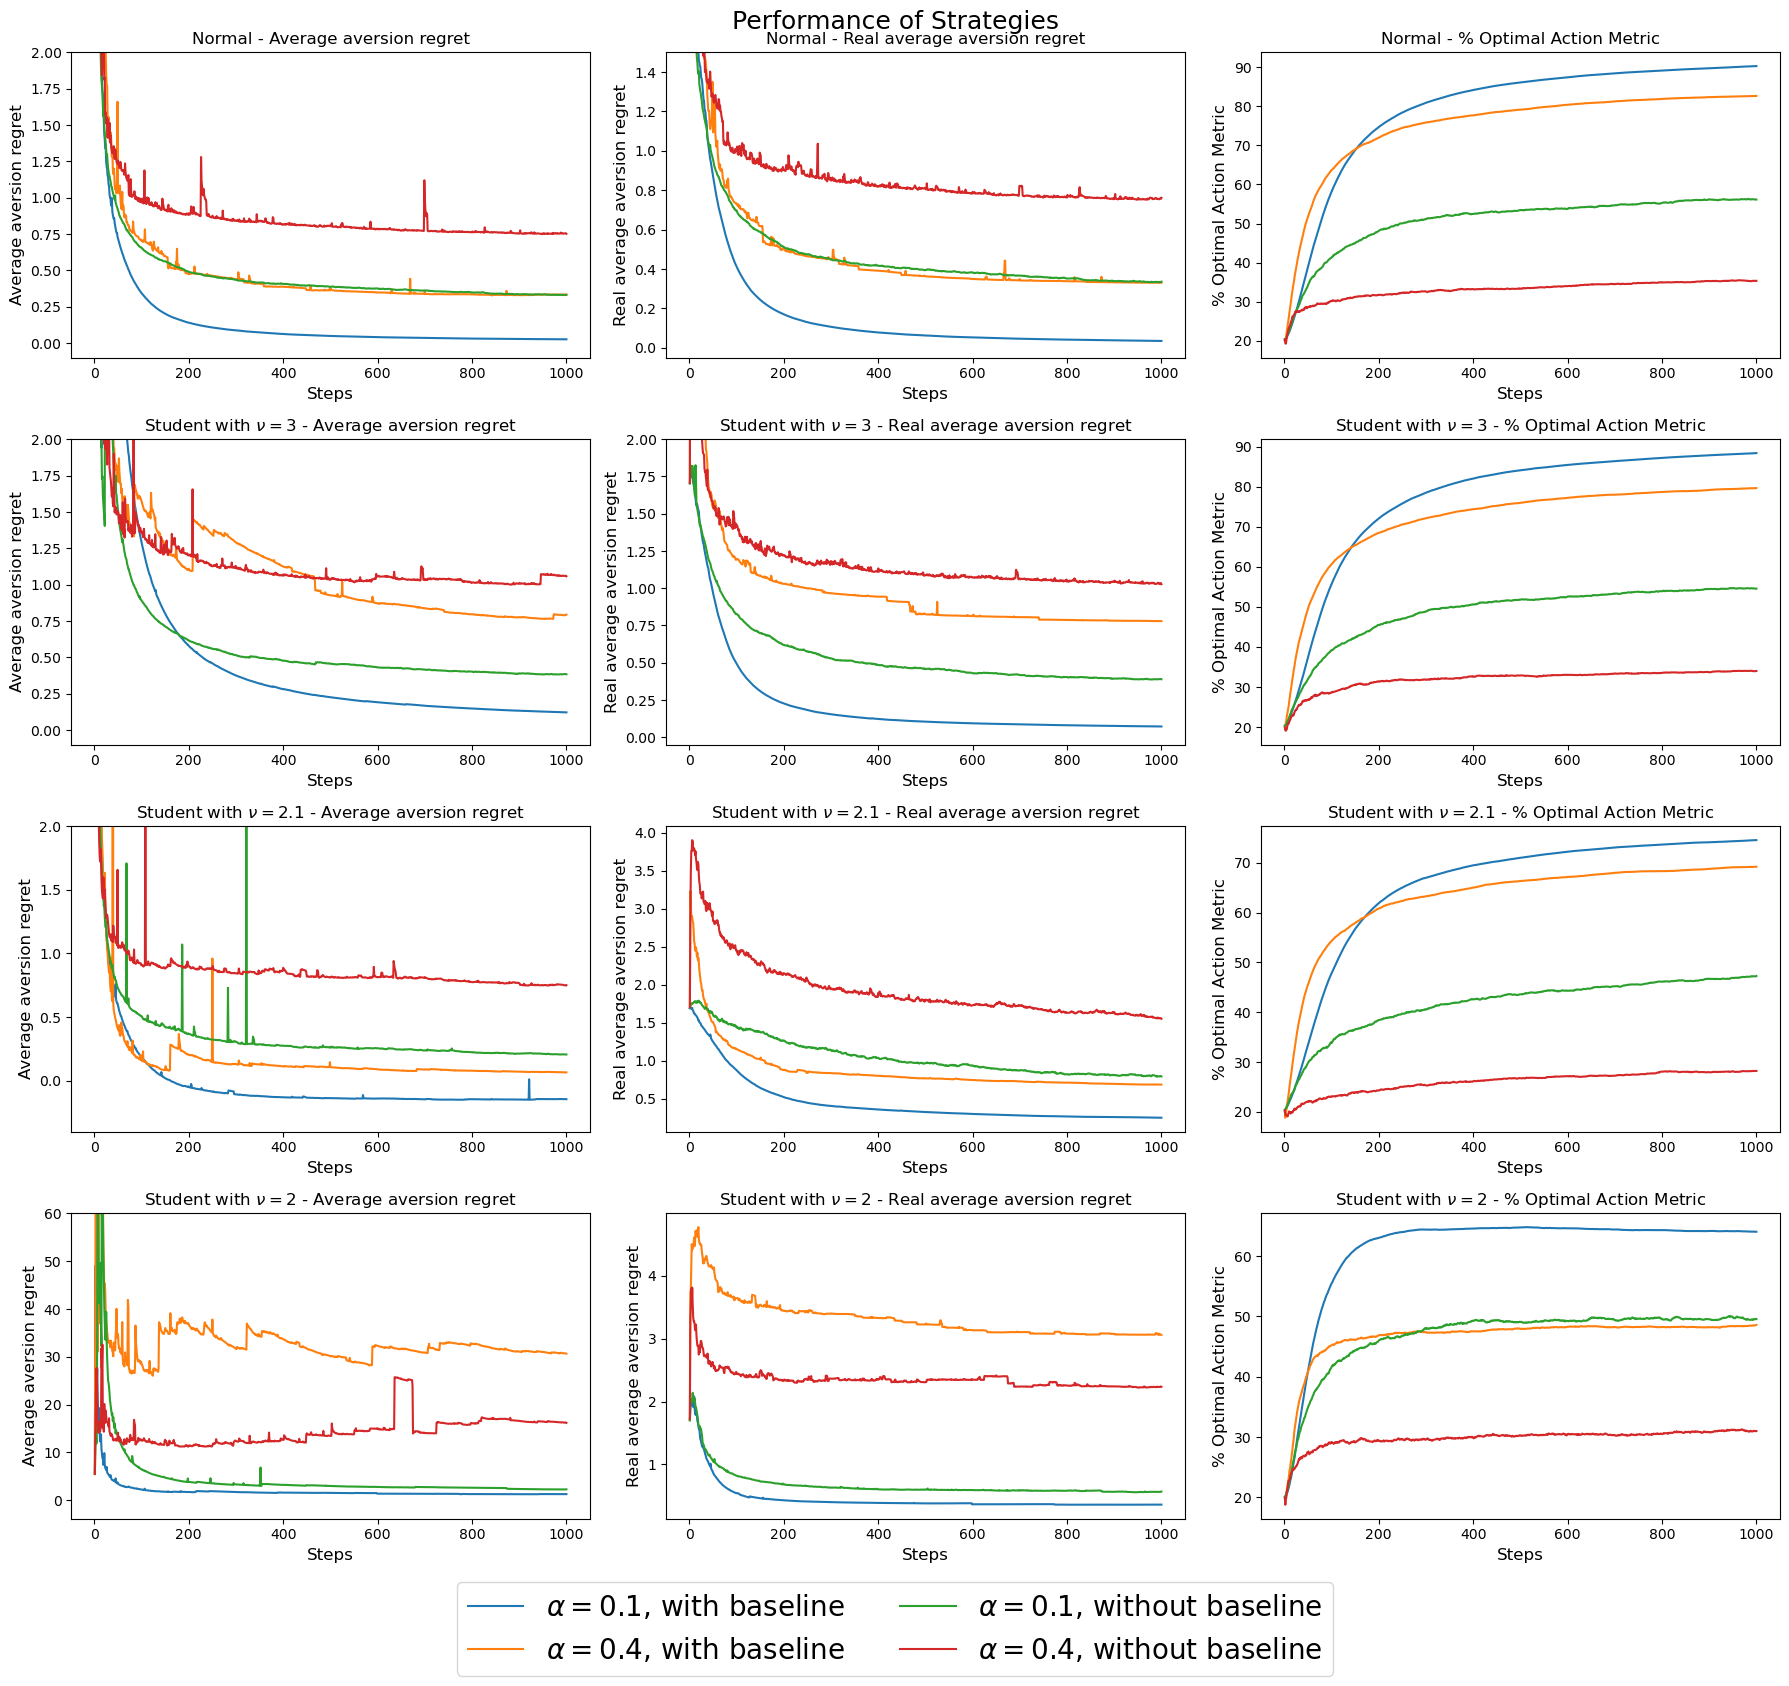
\includegraphics[width=6in]{Figures/experiments_aversion/gradient_bandits/check_strategies_by_distribution.png}
\caption{Графики зависимости метрик количества шагов для различных распределений и стратегий с градментных бандитов с разными baseline и $\alpha$ в измененной задаче}
\label{fig:aversion_gradient_check_strategies_by_distribution}
\end{figure}

Отличный результат для всех метрик показывает, что в теоретической главе был выбран удачный baseline. Результаты по коэффициентам отвращения даны в \ref{fig:aversion_gradient_bandits_last_5_steps}. Результаты улучшают вероятности для реального $\epsilon$-greedy и ухудшают для внутренних вероятностей $\epsilon$-greedy.

\begin{figure}[ht!] %!t
\centering
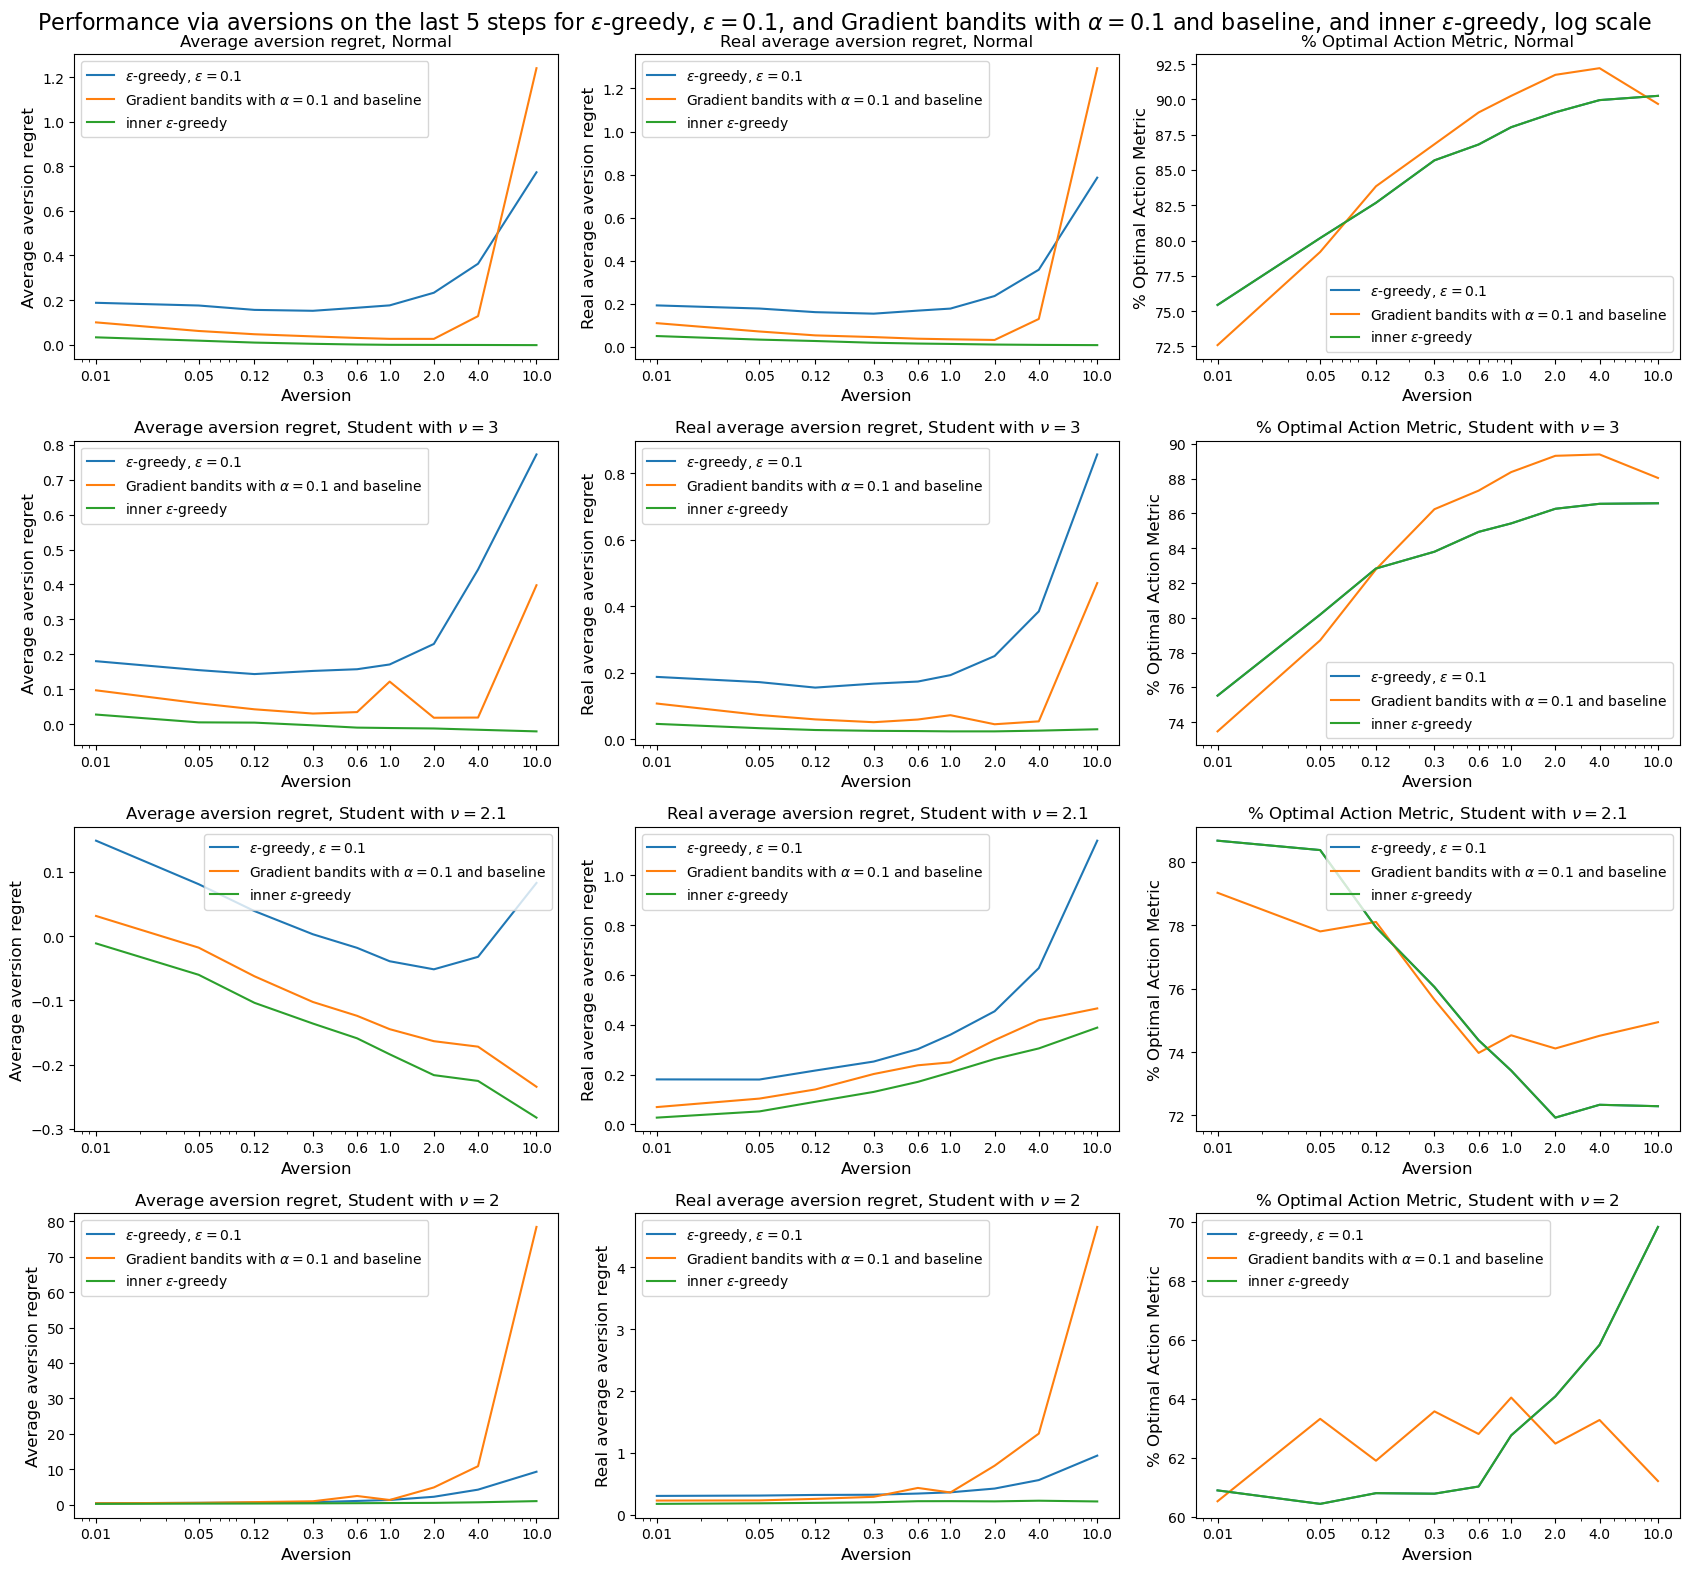
\includegraphics[width=6in]{Figures/experiments_aversion/gradient_bandits/last_5_steps.png}
\caption{Графики зависимости метрик от коэффициента отвращения для распределений и градиентных бандитов.}
\label{fig:aversion_gradient_bandits_last_5_steps}
\end{figure}


\section{Выводы}

По проведенным экспериментам можно сделать следующие выводы:
\begin{enumerate}
    \item Практически все стратегии справляются с достаточно маленькой ошибкой для распределений с большим числом степеней свободы, а именно $\nu \geq 3$
    \item Один из лучших результатов показала простая стратегия $\epsilon$-greedy. Несмотря на то, что внутри себя стратегия хранит вектор вероятностей, очень близко подходящий к оптимальному решению за 1000 шагов, в реальности с вероятностью $\epsilon$ будет выбираться случайный рычаг. Это повышает сожаление стратегии на $0.2$. Поэтому выбор стратегии $\epsilon$-greedy должен основываться на приоритетной цели: если необходимо получить наилучший вектор вероятностей, не считаясь с затратами при обучении, то $\epsilon$-greedy подходит. Если же важна эффективность и на обучении, то лучше рассмотреть другие стратегии, например, градиентных бандитов.
    \item Для $\epsilon$-greedy стратегии при $\nu \geq 3$ эффективность стратегий падает при $\lambda \to 0$. Это связано с проблемой выбора двух рычагов с наибольшими матожиданиями.
    \item Стратегии с адаптивным $\epsilon$ улучшают средний процент оптимальных действий, но никак не влияют на сожаление и среднее сожаление.
    \item Стратегии с жадной позитивной инициализацией и const step-size дают хорошее приближение оптимума при небольшом числе шагов, что может быть полезно, когда результат нужно получить как можно быстрее.
    \item UCB, хотя и обеспечивает понижение среднего реального сожаления, дает ухудшение процента оптимальных действий при больших $\lambda$, поэтому есть смысл использовать UCB только при маленьких $\lambda$
    \item Для градиентных бнадитов применимы те же выводы, что и для UCB.
    \item Для $t_{2.1}$ возникает проблема недооценки дисперсии -- выборочная дисперсия в большинстве случаев сильно занижает реальное значение дисперсии, из-за чего эффективность ухудшается. Это верно для всех стандартных стратегий. Стратегии с корректировкой дисперсии помогают решить проблему, однаок они требуют точного знания значения $\nu$, что не всегда выполнимо в реальной жизни
\end{enumerate}

Как итог, можно сделать общий вывод о том, что при числе степеней свободы, близких к 2, оценка риска через дисперсию слабоприменима.